%--------------------
% Packages
% -------------------

%\usepackage{gentium}
\documentclass[12pt, a4paper]{article}
\usepackage{mathptmx} % Use Times Font
\renewcommand{\baselinestretch}{.92} 
\usepackage[utf8]{inputenc}
\usepackage[margin = 15mm]{geometry}
\usepackage{graphicx}
\usepackage{sidecap}
\usepackage{subcaption}
\usepackage{float}
\usepackage{amsmath}
\usepackage{amsfonts}
\usepackage{amssymb}
\usepackage{array} 
\usepackage{multirow}
\usepackage{tabularx}
\usepackage{pdfpages}
\usepackage{placeins}
\usepackage[title]{appendix}
\usepackage{pdflscape}
\usepackage{booktabs}
\usepackage{gensymb}
\usepackage{wasysym}
\usepackage{multicol}
\usepackage{url}
\graphicspath{{images/}}
 \usepackage{amsmath, amsthm, amssymb}
 \usepackage{array}
 \usepackage{booktabs}
 \usepackage[makeroom]{cancel}
 \usepackage{longtable}
\usepackage{nomencl}
\usepackage{sectsty}
\bibliographystyle{ieeetr}
\usepackage{enumitem} % Includes lists
\frenchspacing % No double spacing between sentences
\linespread{1.2} % Set linespace



%-----------------------
% Begin document
%-----------------------
\begin{document}
\begin{titlepage}
	\centering
    \vspace*{5 cm}
    
\includegraphics[scale = 0.75]{durhamLogo.jpg}\\[1.0 cm]	
    \textsc{\LARGE Maloney's Quay Wall Design Project}\\[2.0 cm]
	\textsc{\Large March 2020}\\[0.5 cm]
	\textsc{\Large Z0983974}\\[0.5 cm]
	\rule{\linewidth}{0.2 mm} \\[0.3 cm]
	\begin{minipage}{0.4\textwidth}
			\end{minipage}~
\end{titlepage}

\section{Executive Summary}
\tableofcontents

\section{Introduction}
\subsection{Site Location}
Maloney's Quay Wall is located on the Tyne River in Newcastle, between Heburn and Bill Quay, as can be seen from Figure \ref{site}. The site lies within the Riverside Park, however access to the site is currently unavailable for the public as a result of the unsafe nature of the wall. Since the wall has collapsed, the wall has been deemed a risk to members of the public, with exposed sharp parts and a potential for other parts of the deck to collapse if people were to walk along it. The nearest residential area is 470m from the wall, and thus this will need to be considered when looking at construction techniques, to ensure that noise disruption is not an issue for the local residents.

\begin{figure}[H]
  \centering
  	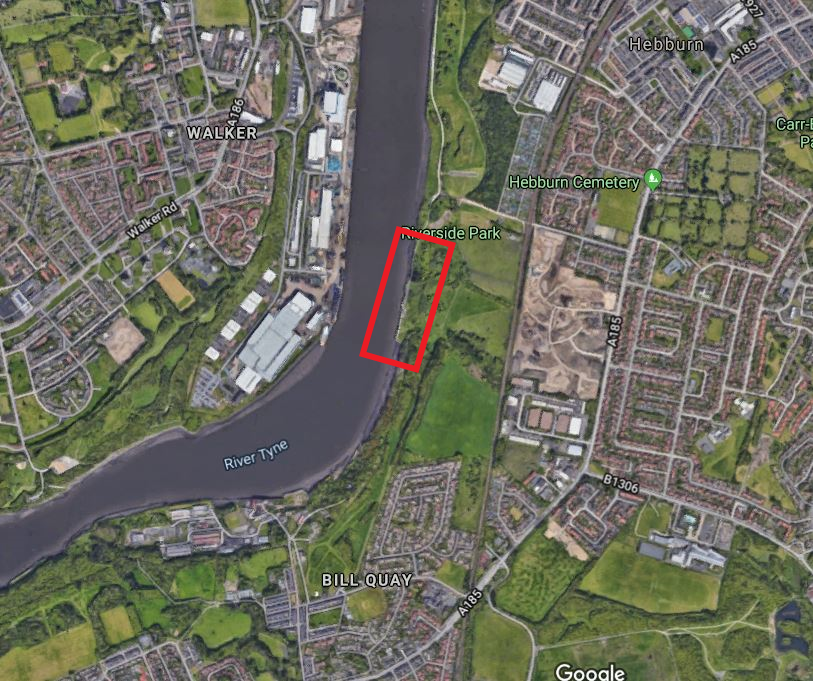
\includegraphics[width=0.5\textheight]{maloneysite}
   	\caption{Aerial Photo of Site Location}
	\label{site}
\end{figure}
\subsection{Site Access}
\begin{justify}
Google Earth was used in this stage of the site analysis to help understand any access restraints, as well as gain a better understanding of the condition and scale of the wall. From Figure \ref{wall}, the main areas of collapse can be seen- a result of buttress erosion from the Tyne river. The area highlighted in red has been identified as a potential location to which a marine rig could be used in the construction phase. However marine rigs can be an expensive and time consuming option, as they are very dependent on the weather conditions and tides. As a result, the marine rig is a last resort option if access via land is not possible. 
\end{justify}
\begin{justify}
With regards to land access, one potential issue is the overgrown nature of the vegetation onto the old access road, identified in Figure \ref{wall2}. However, clearance of this vegetation is an easy solution. Using Google Earth, the access road was measured at the narrowest and widest parts, highlighted in Figure \ref{wall3}- 2.2m and 5m respectively. With the current UK regulations, lorries are limited to 2.55m wide (Road Vehicles (Construction and Use) Regulations
1986 (SI 1986/1078) \cite{a}). There is enough room on the side of the narrowest part of the road to expand slightly, and as shown in Figure \ref{wall2}, smaller lorries have no issue using the road. As a result, land access should not be an issue. In Figure \ref{wall3}, an old car park has been identified as a potential area in which machinery could be stored (circled).
\end{justify}
\begin{figure}[H]
  \centering
  	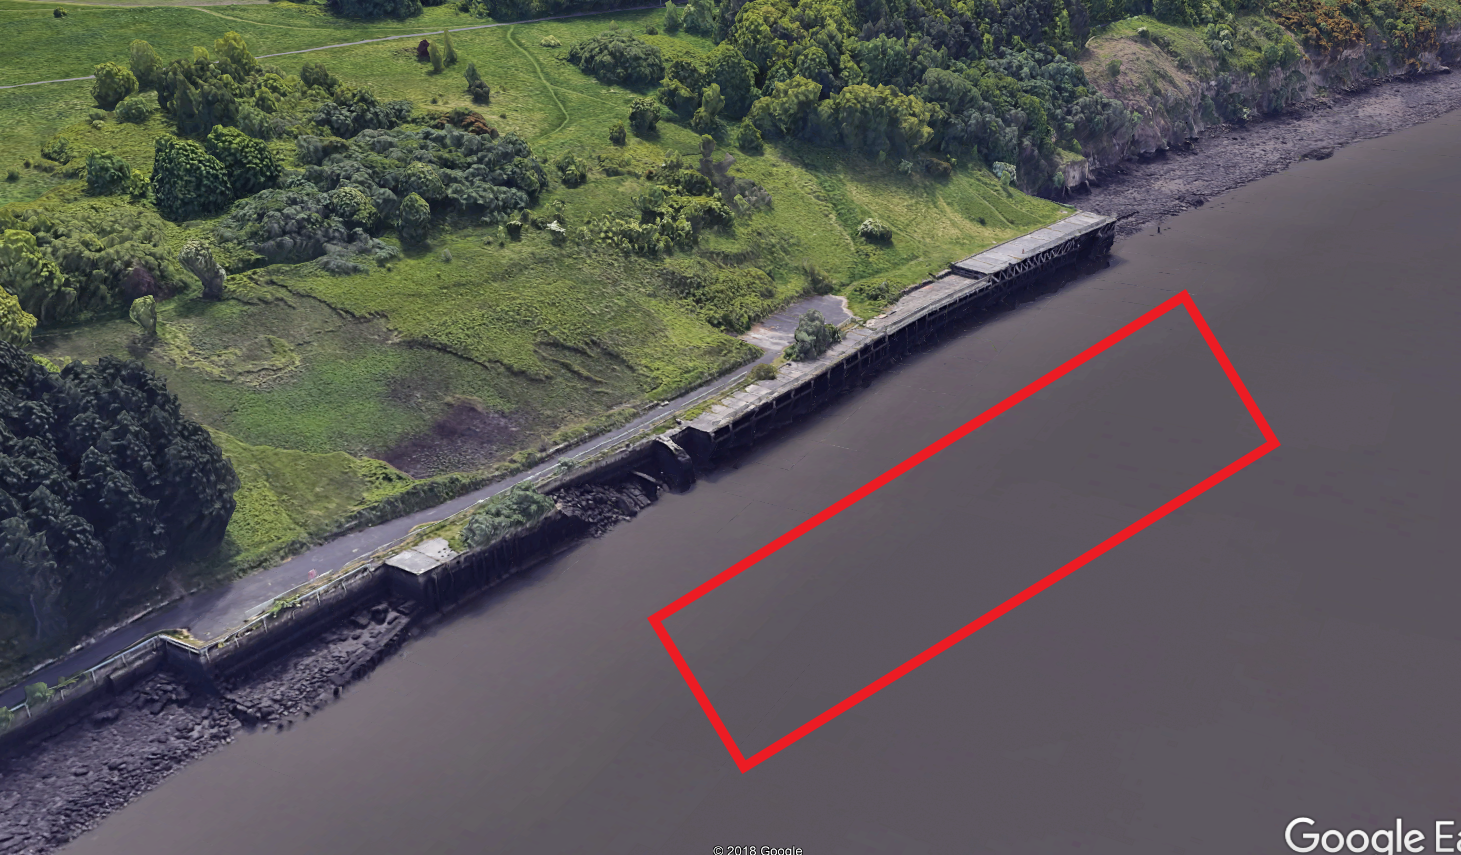
\includegraphics[width=0.5\textheight]{wall}
   	\caption{Aerial photo of wall.}
	\label{wall}
\end{figure}

\begin{figure}[H]
  \centering
  	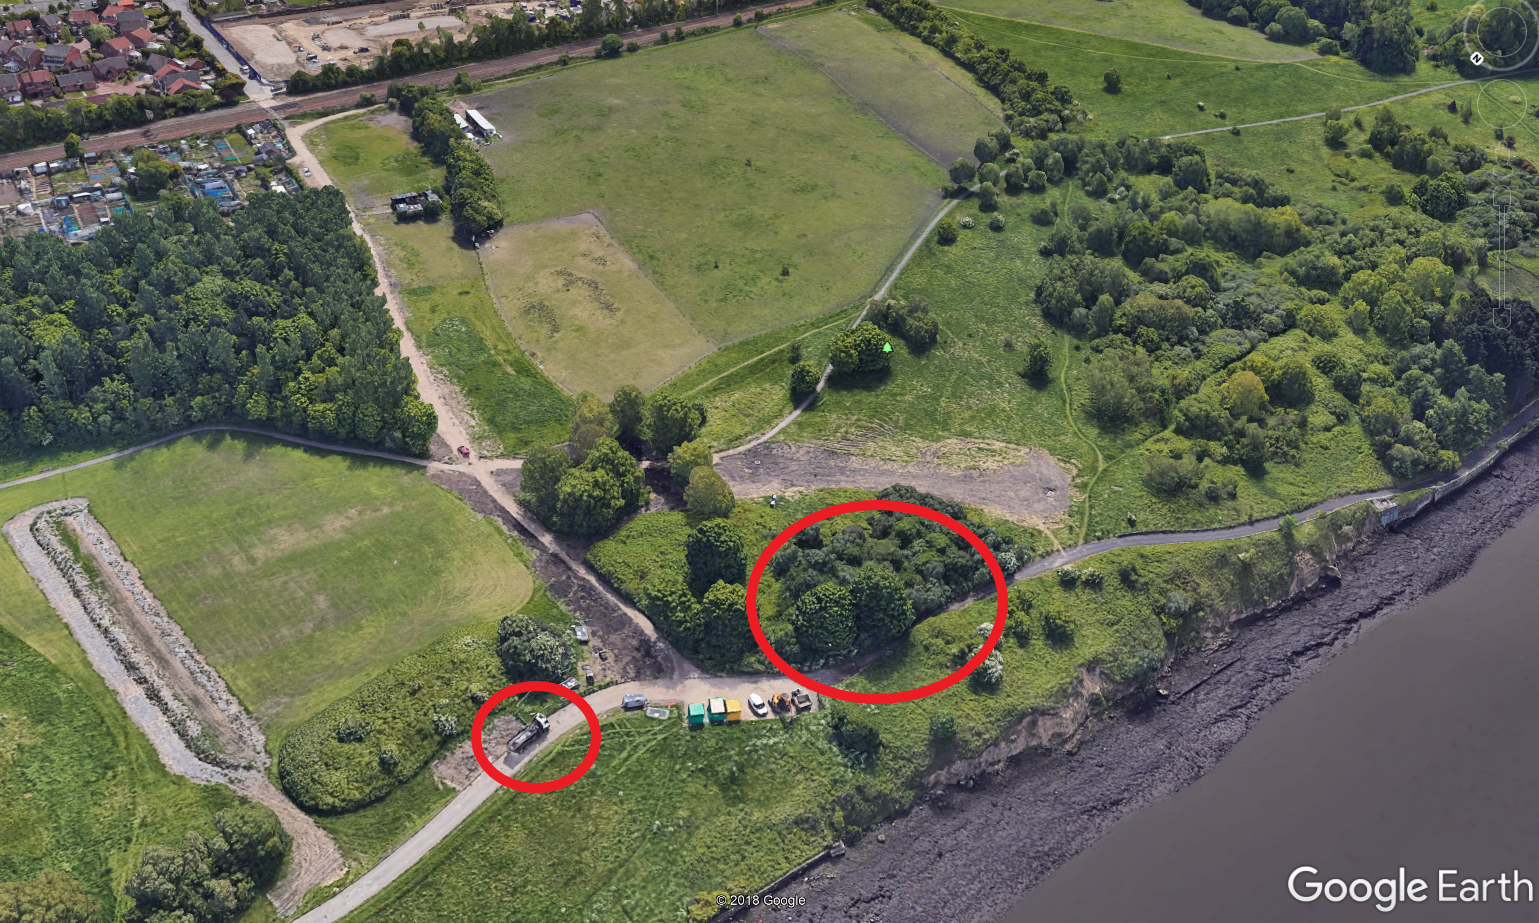
\includegraphics[width=0.5\textheight]{wall2}
   	\caption{Aerial photo of site access constraints.}
	\label{wall2}
\end{figure}

\begin{figure}[H]
  \centering
  	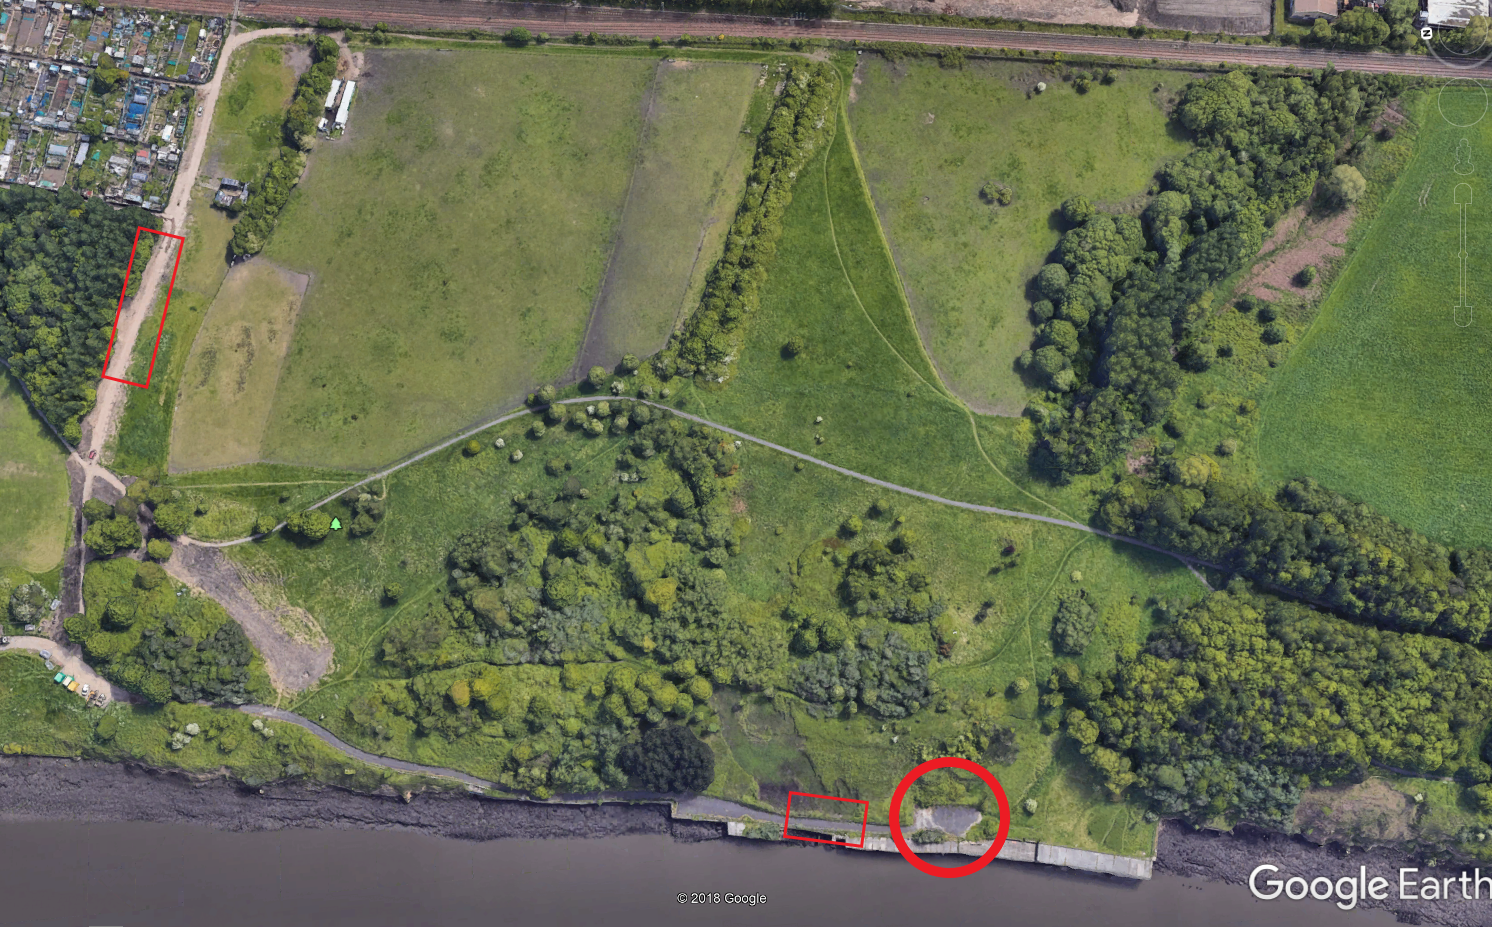
\includegraphics[width=0.5\textheight]{wall3}
   	\caption{Aerial photo showing old car park and road widths.}
	\label{wall3}
\end{figure}
\subsection{Historical Considerations}
The use of the DigiMap Historical map service provided good information on what the wall was used for, and what surrounding industry existed. Going as far back as 1890, it can be seen that the Tyne Copper and Sulphur Works was a large industry operating only 600m North of Maloney's Quay (shown by Figure \ref{hist}. It is likely that the Quay would have been used to load boats with products from this industry, as well as with coal from Hebburn Collary which also used to operate not far from the site. From bore hole data, it has been shown that the waste from this coal industry was buried beneath the ground at this site. This can lead to a process known as `acid mine drainage'. When water interacts with substances such as fool's gold or iron sulphide (typical of waste from coal mining), these substances are oxidised and the result is a very acidic runoff \cite{c}. Wit the site being on the Tyne River, any sudden change to pH can have devastating effect on the marine ecosystems, with Salmon and Sea Trout being the most common fish species in the river potentially at risk. Choosing a wall type which involves the least amount of ground excavation is key, to ensure the chances of uncovering this contaminated land remains small.

\begin{figure}[H]
  \centering
  	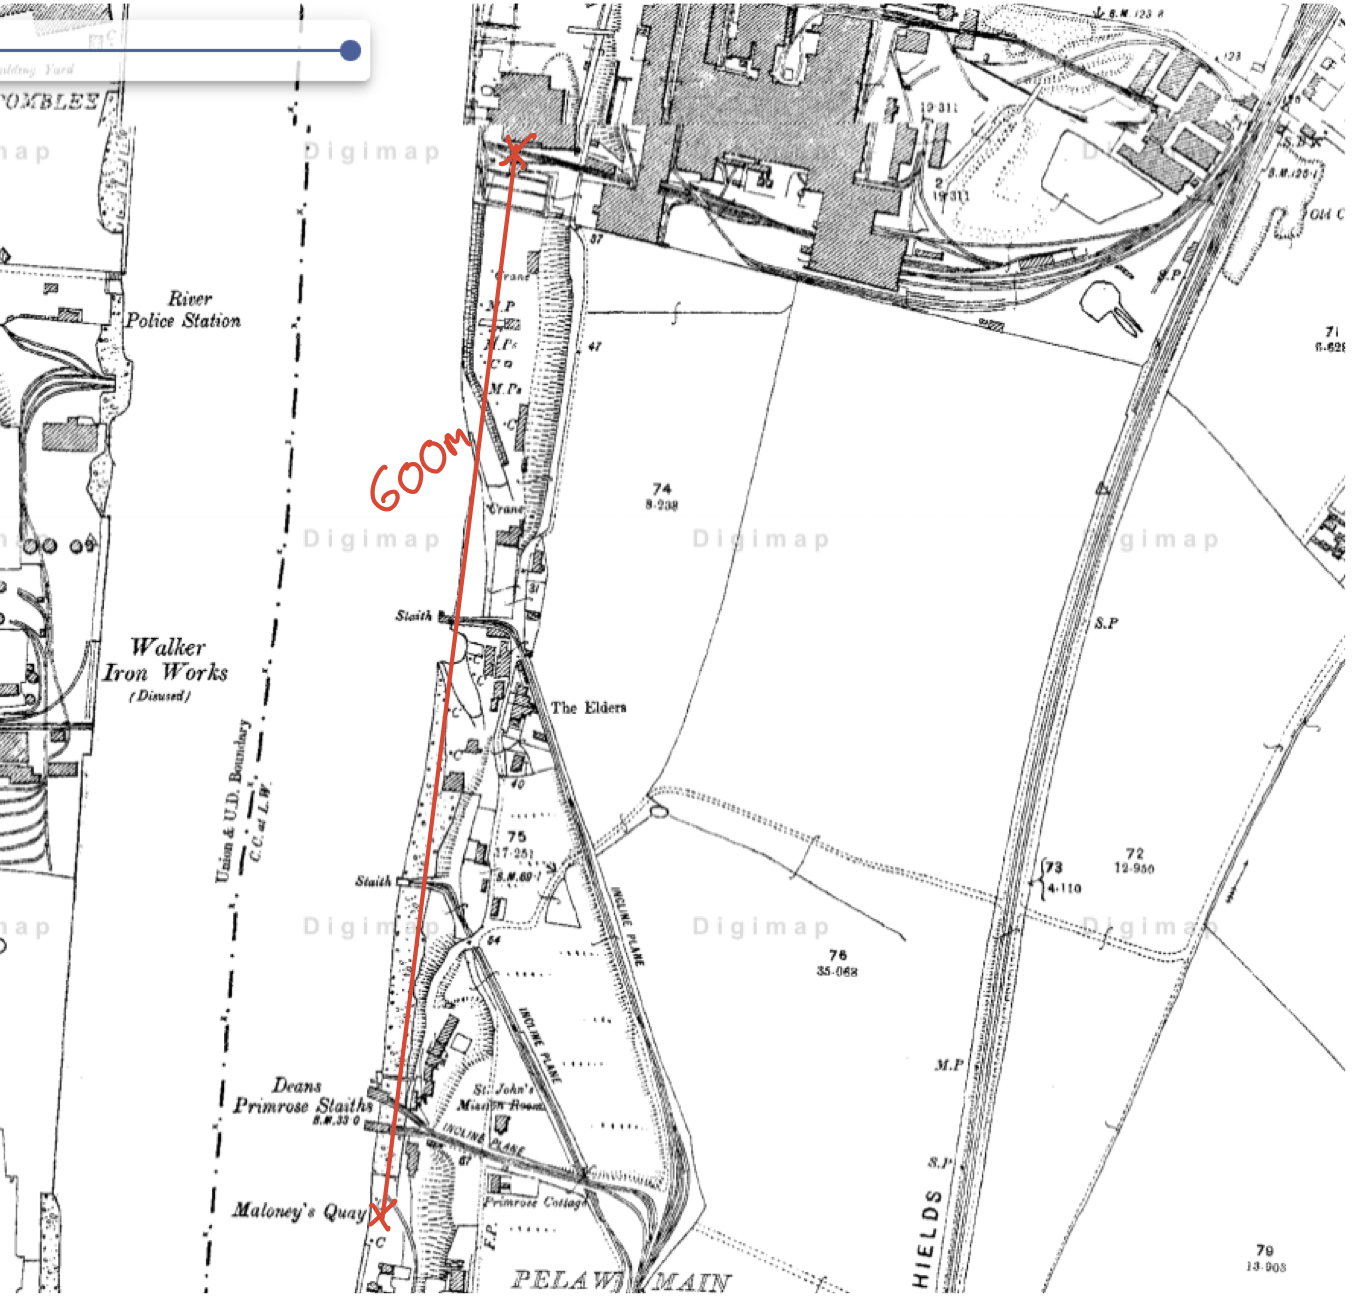
\includegraphics[width=0.5\textheight]{histmap}
   	\caption{Historical Map from 1890 of the site CITE XXX}
	\label{hist}
\end{figure}
\subsection{Site Profile}
As part of the site investigation, understanding the structure of the ground at the site was vital. Various methods were used for this, to gain a complete picture of the site. The British Geological Survey website provided a geology map of the surrounding area to the site, and can be seen in Figure XXX. From this, it is clear that Pelaw Clay is dominant in the area. The project specification provided some useful information on the ground profile, and confirms the Natural Deposits are composed of `soft grey sandy gravelly clay \cite{b}'. From Figure XXX it can be seen that there is boulder clay right on the water side of the wall which will have to be a consideration when considering driving piles. There is a potential for random boulders to appear in the ground, which can be very difficult to penetrate with driven sheet piles.
\begin{figure}[H]
  \centering
  	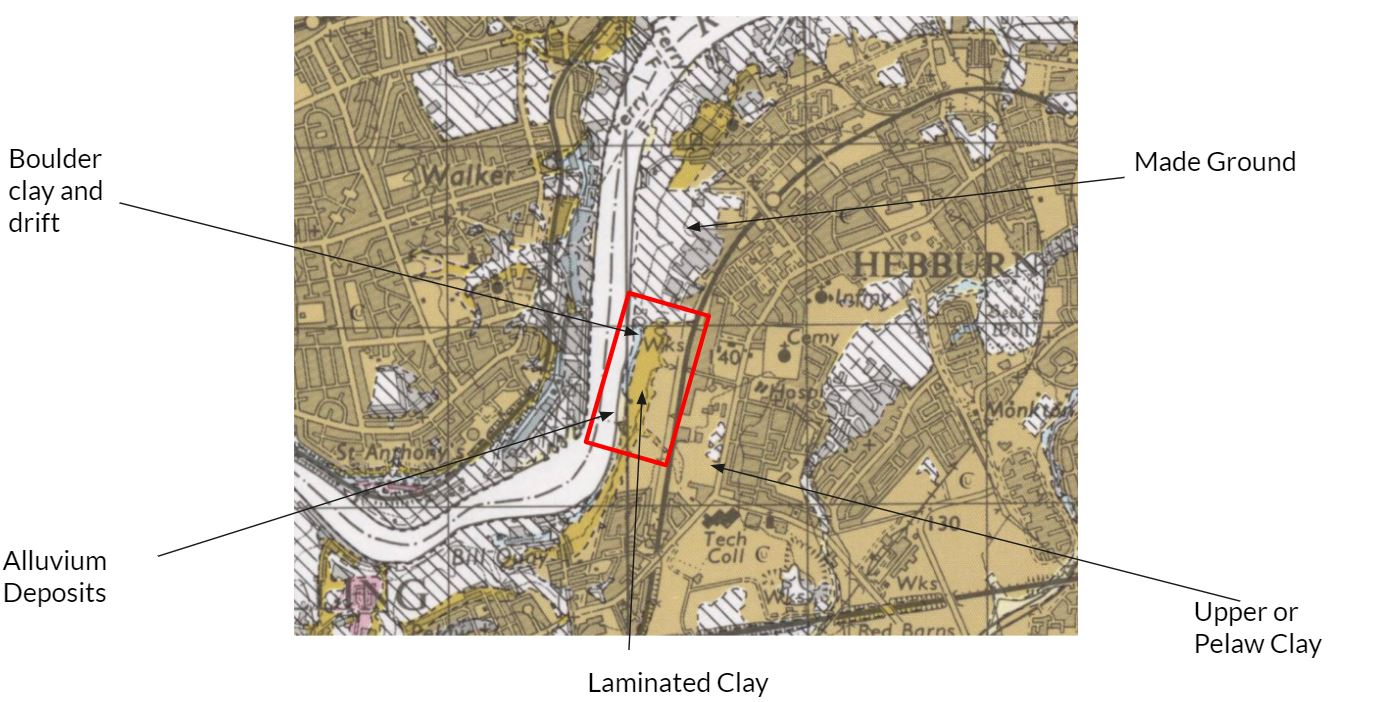
\includegraphics[width=0.5\textheight]{goodgeomap}
   	\caption{}
	\label{length}
\end{figure}

\begin{justify}
The specification provided good information on how the geology changes as you go further inland, however it provides no information on how the geology changes as you travel along the length of the wall. The bore hole data found on the BGS website was used to map a potential ground model. In Appendix A, a screenshot from the BGS website shows the bore holes used to sketch a rough model of the ground profile, shown in Figure \ref{length} in Appendix A. The main points identified from this is that there is a consistent layer of Made Ground along the length, ranging from 2.5-10 feet in depth. Beneath this layer there is mainly variations of clay. At site '1', the shaded in section of the profile (in green), indicate a glacial boulder. These random boulders could be an issue for driving sheet piles into the ground. However, the fact that these boulders only appear to the North of the site and away from the actual wall, suggest that they should not pose an issue for construction.  
\end{justify}
\section{Wall Options}
\begin{justify}
There are various types of retaining wall, all capable of fulfilling the requirements of this project. Some types will do a better job than others however, and thus it was important to research the main types, looking at the advantages and disadvantages of each type. The main types of wall are summarised below. 
\end{justify}
\subsection{Gravity walls}
\subsubsection{Mass Gravity Wall}
\begin{justify}
This type of wall relies on its self-weight alone to provide resistance to the lateral earth pressure. Large sections of concrete, often poured off site, are used to hold the material behind it. These walls require large ground excavation to occur to allow for the wall to sit firmly in the ground, and thus is not an ideal option due to the contamination within this site. These walls can have steel reinforcement added to increase the strength of the wall and reduce the amount of concrete required.
\end{justify}
\subsubsection{Cantilever Gravity Wall}
\begin{justify}
The cantilever wall is similar to the mass wall in terms of the construction process, however the shape of the wall is very different. The cantilever wall's main body is a lot thinner, and has a `heel' and `toe' extending from the base of the wall. These parts of the wall are then buried beneath the ground, and provide additional resisting moments, to stop the wall from overturning. This type is more economical as less concrete is required. However, the design is more complicated and off site construction is required. With site access limited, this may be an issue. For both of these gravity walls, the total removal of water is required for construction, and thus the use of cofferdam may be required, increasing project costs.
\end{justify}
\subsection{Embedded Walls}
\subsubsection{Sheet Piles}
These walls are constructed from sheets of steel, made in either Z or U shaped sections, which are then connected to form a wall. These steel sections are driven deep into the ground, often using a hydraulic press or vibratory rig. If the wall is to be embedded in a hard rock, pre-auguring of the rock is often required to allow for the wall to be embedded. This option is attractive for this design as no excavation is required for embedment. It is also possible to construct the wall without creating a dry environment. One issue with this type of wall is that the embedding process of the wall can cause a lot of noise, potentially disturbing nearby residents. 
\subsubsection{King Post}
\begin{justify}
This type of wall relies on the vertical insertion of H-beams into the ground. Concrete slabs are then slid in between these H-beams, forming the wall. These walls are good for sites where it is beneficial to construct the wall on site, when site access is limited. King Post walls are virtually vibration-less in construction and thus noise disruption is minimal. They also do not required any excavation and thus no spoil is created, vital in a site such as this.
\end{justify}
\subsubsection{Bored Piles}
\begin{justify}
There are three main types of Bored Pile wall, the first of which is the Contiguous Pile Wall. These are concrete piles, cast on site at regular intervals, leaving gaps between each pile. These are the cheapest option of all three bored piles, but the least efficient, as they are unable to retain water, thus rendering them useless for the required design. 
\end{justify}
\begin{justify}
The second type is the Secant Wall- Hard/Soft. This option is used where short term water retention is required. Soft concrete piles are installed first, with the harder reinforced secondary piles installed in the gaps between the primary ones. This is done by either a rotary auguring process or CFA techniques, where the sides of the primary piles are drilled into as the secondary piles are poured. This wall is not a water tight solution, however water flow is reduced greatly. However, water retention is only short term as the soft piles can shrink, leading to gaps where water can seep through. 
\end{justify}
\begin{justify}
The third type is the Secant Wall-Hard/Hard. This is where both the primary and secondary piles are made from reinforced concrete, making a long term water retention solution.
\end{justify}
\subsection{Rock/ Ground Anchors}
\begin{justify}
Rock or ground anchors are a solution that can be combined with any of the above wall types, to increase the retaining strength of the wall. A rock anchor is where a steel tie rod, often at an angle, connects the wall to an anchor which is grouted into the rock. A ground anchor is where a tie rod connects the wall to either a concrete block (dead man anchor) or a short sheet pile, further back from the actual wall. Anchors are most commonly used with sheet piles, where it is often preferable to reduce the embedment depth. The deeper a wall is to be embedded, the more time consuming and costly the project will be. By adding either a rock or ground anchor, the wall does not need to be as deep to offer the same resistance, due to some retaining force coming from the anchor.
\end{justify}
\begin{justify}
Having researched the above wall options, a design matrix was created to help analyse the best solution for the project requirements, and can be seen in Appendix XXX. From this matrix, it was found that Sheet Piles were the most preferable for the final design. 
\end{justify}
\section{Initial Sheet Pile Depth Calculations}
\subsection{Soil Parameters}
\begin{justify}
The design characteristics for the soils at the site are shown below in Table \ref{param} and were used throughout the design process. Using DA1.C2 from Eurocode 7, a partial factor of 1.25 was used for to scale down both the cohesion factor (c') and the angle of shearing resistance (tan$\phi$)
 
\end{justify}
\begin{table}[H]
\centering
\begin{tabular}{|c|c|c|c|c|c|c|c|c|c|}
\hline
     \textbf{Soil Type}& \textbf{$\gamma$/kN/m$^3$}& \textbf{$\phi$'/$\degree$}&\textbf{$\phi_w$'/$\degree$}&K$_{a1}$&K$_{a2}$&K$_{p1}$&K$_{p2}$&c'&c$_w$'\\ \hline
      1 (Sand Unsaturated)&17&24.8&16.5&0.36&/&/&/&0&0  \\ \hline
      2 (Sand Saturated) & 19.5&24.8&16.5&0.36&/&/&/&0&0  \\ \hline
      3 (Sandstone) & 23 &28.4&18.9&0.32&1.06&5.34&6.38&8&0 \\ \hline

\end{tabular}
\caption{Soil Parameters used in calculations.}
\label{param}
\end{table}
\subsection{Bending Moments in Sheet Pile}
\subsubsection{Without Anchor}
\begin{justify}
The horizontal effective pressures at each significant level (3m,6.4m and at the toe of the wall), were calculated, and the results are shown in a screen capture of the original spreadsheet used, in Appendix XXX. The equations that underlie these results are shown below (Equation XXX, XXX
\end{justify}
\begin{equation}
 \sigma_{v}=\gamma z   
 \label{sigv}
\end{equation}

\begin{equation}
    \sigma'_v=\sigma_v-u
    \label{sigvdash}
\end{equation}

\begin{equation}
    \sigma'_{h(cohesionless)}=Ka_1 \sigma'_v
    \label{horizstresscohesionless}
\end{equation}
    
\begin{equation}
      \sigma'_{h(cohesion)}=Ka_1\sigma'_v-c'Ka_2
      \label{horizstresscohesion}
\end{equation}
\begin{justify}
Having obtained the horizontal effective stress at each level where the soil property changes, they could be plotted on a diagram as shown in Figure \ref{pressdiag}. From this, the forces from each section, labelled 1 to 9, could be calculated by calculating the area of the section. The force acts through the centroid of the shape-midway for the rectangles, and a distance of 1/3 the height from the base for the triangles.
\end{justify}

\begin{justify}
Knowing all the forces and the point at the which they act, moments were taken about the toe of the wall, at an assumed initial depth. The overturning moments and restoring moments were calculated, and the factor of safety was found using Equation \ref{fos}.  Having already accounted for the partial safety factor for c' and tan$\phi$', and taken a safety factor of 1.3 to the surcharge load (also advised by DA1.C2 Eurocode 7), the FoS for overturning only had to equal 1.0 or above.
\end{justify}
\begin{equation}
    FoS=\frac{\textsc{restoring moment}}{\textsc{overturning moment}}
\label{fos}
\end{equation}


\begin{figure}[H]
  \centering
  	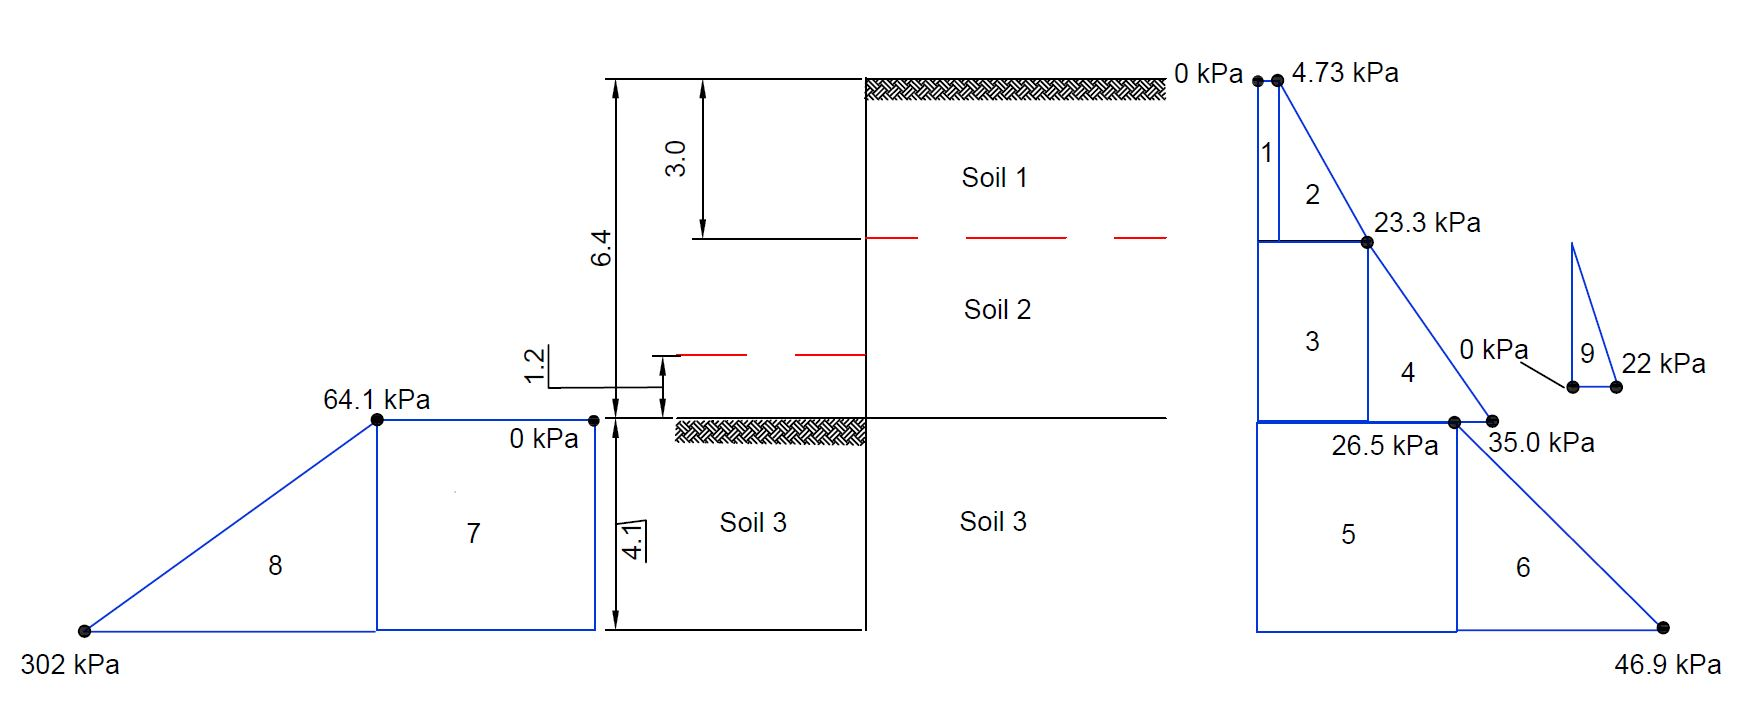
\includegraphics[width=0.7\textheight]{initialwallcalcsmodel}
   	\caption{}
	\label{pressdiag}
\end{figure}
\begin{justify}
Using the excel spreadsheet, an iterative process was used to find the depth of the wall that allowed for such a factor of safety. It was found that a penetration depth of 4.3m into the rock gave a FoS=1.1.
\end{justify}
\begin{justify}
Having calculated the required depth to stop overturning, a bending moment diagram was created. Using Figure \ref{bendmomfig}, Table XXX in Appendix XXX was created. The segments are at 1m intervals (apart from segment 7,8 and 12), and the force was calculated from the area of the trapezium. The location of the force was calculated using Equation \ref{y} below, to calculate the centroid location y-metres from the base of the trapezium. From this, the moment about the top of the wall at each trapezium was calculated. Where there is a trapezium with the same numbering as another, the values of moments are summated, taking into account the direction. The moment at each 1m interval was then plotted to produce the bending moment diagram shown in Figure XXX.
\end{justify}

\begin{equation}
    y=\frac{h(b+2a)}{3(b+a)}
    \label{y}
\end{equation}

\begin{figure}[H]
\centering
  	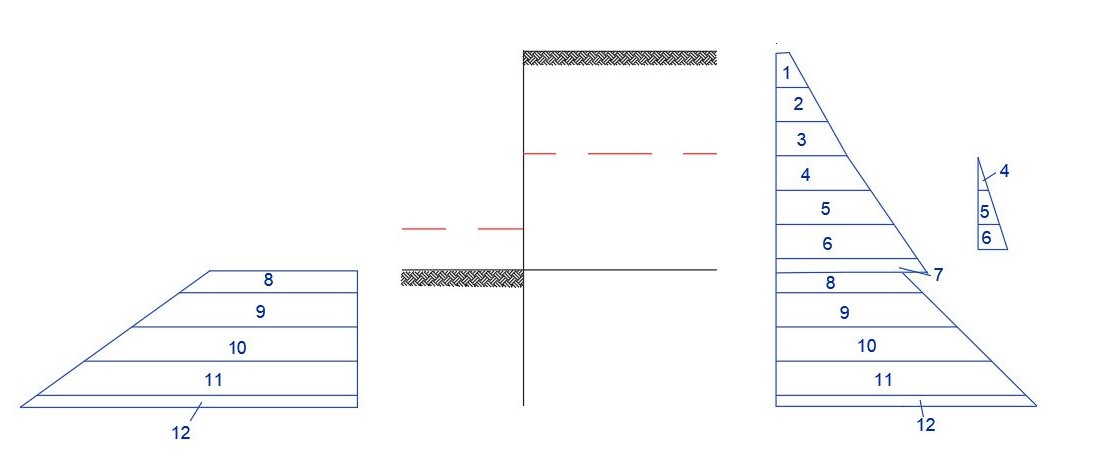
\includegraphics[width=0.75\textheight]{bendingmomentcalcsfig}
   	\caption{Passive Soil Pressure Calculations}
	\label{bendmomfig}
\end{figure}

\begin{figure}[H]
\centering
  	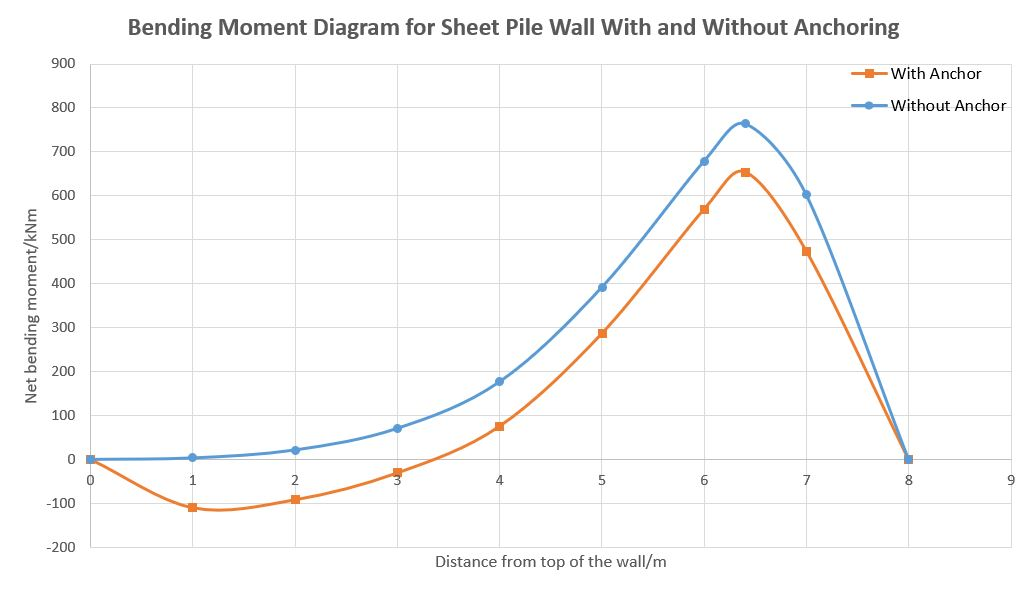
\includegraphics[width=0.6\textheight]{bmdiag}
   	\caption{Bending moment diagram for sheet pile with anchor and with no anchor.}
	\label{bendmomdiag}
\end{figure}
\begin{justify}
From Figure \ref{bendmomfig} it can be seen that the maximum bending moment is 764 kNm and occurs at the point at which the passive resistance starts (6.4m below the top of the wall). The bending moment diagram plotted is only plotted up to 8m below the top of the sheet pile because beyond this, the bending moments become negative and are of no interest.
\end{justify}
\subsubsection{With Anchor}
\begin{justify}
The next stage of design was to try and minimise the depth at which the sheet pile was required to be at. This meant involving an additional horizontal retaining force on the sheet pile in the form of an anchor. It was initially assumed that a ground anchor was to be used, acting at a depth of 1m from the top of the wall. The required anchor force was calculated by finding the difference between the forces acting to the right and the forces acting to the left. Obviously this would depend on the depth at which the wall went to, and thus an iterative process was required. The use of Excel meant that everything was interconnected and made updating values much easier.
\begin{justify}
The initial overturning and restoring moment calculations were done again, this time taking the moments about the Tie Force location. The depth of the wall was then adjusted to obtain a FoS greater than 1.0. This time around, a wall depth of 2.4m provided a FoS=1.03. The Bending Moment diagram with the anchor involved, shown in Figure \ref{bendmomdiag}, was then obtained using the same technique as before, making sure to account for the moment from the Tie Force. 
\end{justify}
\begin{justify}
It can be seen that the anchor not only reduces the required embedment depth by 44\%, but also reduces the maximum bending moment in the sheet pile by 14.4\%. These will reduce the overall project cost in when it comes to implementation. It takes less time to embed the wall to a shallower depth, and a weaker sheet pile will be required to cope with the smaller bending moment, which will be cheaper than a stronger section. 
\end{justify}
\end{justify}
\begin{justify}
Having found the maximum bending moment in the wall, a section capable of withstanding this moment could then be chosen for the wall. It was assumed that S430 Steel was to be used, meaning the stress of the section at maximum bending moment had to be less than 374 MPa (applying a safety factor of 1.15 to yield stress). Through an iterative process and using Equation \ref{stresspile}, it was found that an Elastic Section Modulus of 1800cm$^3$/m would satisfy the requirements. From this it was decided that an AZ-18-700 section would be satisfactory in withstanding the maxmimum bending moment. 
\end{justify}
\begin{equation}
    \sigma=\frac{M_{max}}{Z}=\frac{654000}{0.0018}=363 MPa < 374 MPa
    \label{stresspile}
\end{equation}
\section{Anchor Wall Calculations}
The next part of the design was calculating the required size of the anchor wall, as well as where it the anchor wall is to be embedded. The general concept was to embed a sheet pile further behind the front wall, and connect it to the wall with tie rods, to provide further resistance to the active pressure of the soil behind the wall. 
\begin{justify}
A similar approach to the previous method of calculating the overturning and restoring moments was used for the anchor wall. In Appendix XXX, the tables used in excel are shown. In Figure \ref{anchor1}, Kac and Kpc were calculated using Equation XXX below. Layer 1 and 2 are the clayey fill and the sandstone respectively. It was assumed for these calculations that the anchor wall would not exceed a depth of 8m. 
\end{justify}
\begin{equation}
    K_{ac}=2\sqrt{K_a(1+\frac{a}{c})}
\end{equation}
\begin{equation}
     K_{pc}=2\sqrt{K_p(1+\frac{a}{c})}
\end{equation}
\begin{justify}
In Figure \ref{anchor3}, the horizontal effective stress was calculated as before using Equation \ref{horizstresscohesionless} and \ref{horizstresscohesion}, where Ka$_2$ is equivalent to K$_{ac}$/K$_{pc}$.
\end{justify}
\begin{justify}
In Figure \ref{anchor5}, the moments are then taken about the toe of the anchor wall, at an assumed depth of the anchor wall, using the same method as with the main wall. The anchor force is accounted for at this point, previously calculated. It is vital that the restoring moment is larger than the overturning moment, and thus this ratio was calculated. An iterative process was then carried out, changing the depth of the anchor wall to ensure the ratio was greater than 1. Equation \ref{wallfos} shows that the depth of 2.8m achieved this.
\end{justify}
\begin{equation}
      FoS=\frac{\textsc{restoring moment}}{\textsc{overturning moment}}=\frac{213}{203}=1.05>1
      \label{wallfos}
\end{equation}
\begin{justify}
It was then required to ensure that not only was the anchor wall in equilibrium in terms of moments, but also in terms of horizontal forces. With the horizontal forces  shown in Figure \ref{anchor5}, there was a greater force from the passive side. To calculate the net passive resistance force required to fix the toe of the pile, Equation \ref{p12} was used in conjunction with Figure \ref{anchorwall}.
\end{justify}
\begin{equation}
    (P2+P3)= P1-T=229-113=116N
    \label{p12}
\end{equation}
\begin{justify}
Following this, the depth at which this force could be achieved was calculated, shown in Figure \ref{anchor6}. A value of d2=0.7 led to a force of:
\begin{gather}
    (P2+P3)=133N >116N
\end{gather}
 
\end{justify}
\begin{justify}
The total depth of the anchor wall required is equal to:
\begin{gather}
    \text{Total Anchor Depth}= d1+\Delta=2.8+0.84=3.64m
\end{gather}
where $\Delta$=1.2 x d2.
\end{justify}

\begin{figure}[H]
\centering
  	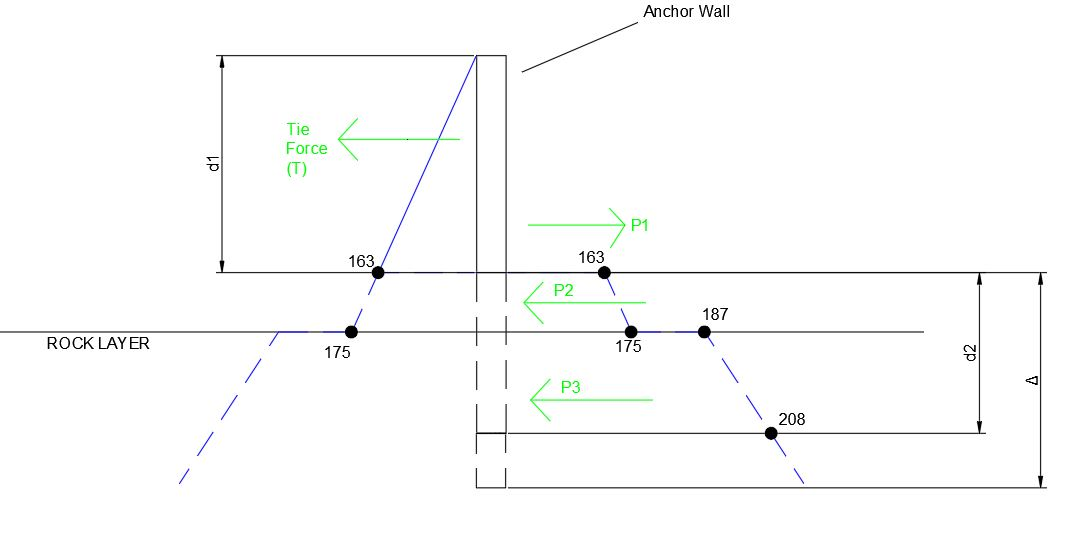
\includegraphics[width=0.6\textheight]{anchorwallfig}
   	\caption{Diagram used in calculating required anchor wall depth.}
	\label{anchorwall}
\end{figure}


\begin{justify}
The next task was to calculate the location of the anchor. It is required that the anchor lies outside of the the plane YZ, seen in Figure \ref{anchor}, `to ensure that the passive wedge of the anchor does not encroach on the active wedge behind the wall \cite{e}'. Knowing the length of wall required to be outside plane YZ, and the angles given, it was a simple case of trigonometry to calculate the required distance between the back of the main wall and the front of the anchor wall. This value is 13m.
\end{justify}

\begin{figure}[H]
  \centering
  	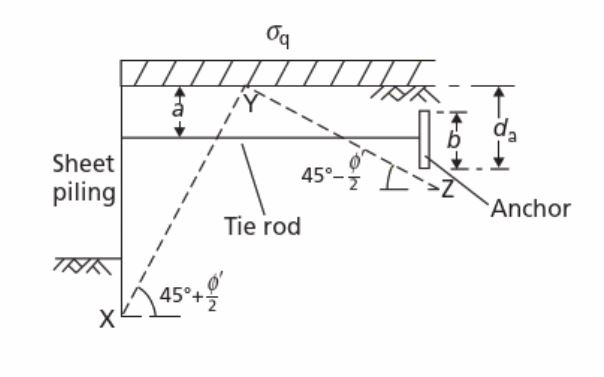
\includegraphics[width=0.5\textheight]{pilinghandbooktie}
   	\caption{Diagram to explain the method used in determining the location of the anchor wall. \cite{e}}
	\label{anchor}
\end{figure}

\section{Waling Wall Design}
\subsection{SLS Checks}
\begin{justify}
The next task was to find an appropriate section for the waling wall, that could withstand the forces and bending moments in the sheet pile. The maximum bending moment in the waling wall was calculated using Equation \ref{m}. 
\end{justify}
\begin{equation}
    M=\frac{Fl^2}{10}=\frac{113 \times 2.8^2}{10}=88kNm
    \label{m}
\end{equation}
\begin{justify}
From this, the required elastic modulus was calculated, using Equation \ref{wy} and assuming S430 steel would be used. 
\end{justify}
\begin{equation}
    W_y=\frac{M}{f_y}=\frac{88 \times10^3}{430}=204.7 cm^3
    \label{wy}
\end{equation}
\begin{justify}
As there are two Parallel Flange Channels (PFC) required to make the waling wall, this required elastic modulus is halved. It was then required to find a PFC section with an elastic modulus greater than 102.3 cm$^3$. PFC 150 x 90 x 24 has an elastic modulus of 155 cm$^3$. To find the Utilisation Factor (UF), Equation XX was used.
\end{justify}
\begin{equation}
    UF=\frac{102}{155}=66\%
\end{equation}
\begin{justify}
The flange thickness for this section is 12mm. Assuming a loss of 1.2mm in thickness to each face after 50 years, due to corrosion in a non compacted and non aggressive fill \cite{h}, this leads to a total loss of 2.4mm to the flange thickness. Equation \ref{strengthloss} assumed this thickness loss is proportional to the loss in strength.
\end{justify}

\begin{equation}
\text{Loss of strength}=\frac{2.4}{12}=20\%<34\%
\label{strengthloss}
\end{equation}

\begin{justify}
From the above equation, it can be seen that there is a 14\% additional capacity in the SLS.
\end{justify}
\subsection{ULS Checks}
\begin{justify}
Using the data sheet from British Steel \cite{f}, the second moment of area I$_y$ was found, shown below. The reduced second moment of area, assuming a loss of 1.2mm to every face due to corrosion after 50 years, was calculated using an online software called SkyCiv. 
\end{justify}

\begin{justify}
\hspace*{8cm}
I$_y$=1162 cm$^4$ \\
\hspace*{8cm}
I$_{y, red}$=898cm$^4$
\end{justify}
\begin{equation}
    \text{Double Channel:}=2 \text{x} 898=1797cm^4
\end{equation}
\begin{equation}
    W_{el,red}=\frac{I_{y,red}}{y}=\frac{1797}{14.76/2}=243.5 cm^3
    \label{welred}
\end{equation}
\begin{justify}
The value of y in Equation \ref{welred} was taken as half the reduced total height of the section. The next stage was to work out what Class the waling section was. 
\end{justify}
\begin{equation}
    \epsilon=\left(\frac{235}{f_y}\right)^{0.5}=\left(\frac{235}{430}\right)^{0.5}=0.739
\end{equation}
\begin{equation}
    \frac{c}{t_f}=\frac{83.5}{12}=6.96
\end{equation}
\begin{equation}
    \frac{c}{t_f}<10\epsilon \implies \text{CLASS 2}
\end{equation}
\begin{justify}
As this section is Class 2, the plastic section modulus can be used for bending resistance verification. However, there is no data for the reduced section for plastic section modulus, and so the reduced elastic section modulus is used instead. This is a conservative trade-off, as the elastic section modulus is smaller than the plastic, and thus if the bending resistance is larger than the maximum moment in the waling wall when using the elastic modulus, it will definitely be larger if the plastic section modulus had been used.
\end{justify}
\begin{equation}
    M_{c,Rd}=\frac{W_{el,red}f_y}{\gamma_{M0}}=\frac{243.5\times430}{1}=104.7kNm>88kNm \hspace*{1cm}\text{(from SLS check)}
    \label{mcrd}
\end{equation}
\begin{justify}
From Equation \ref{mcrd}, it is shown that even after 50 years of corrosion, the waling wall's bending resistance remains larger than the maximum bending moment in the waling wall and thus the PFC 150 x 90 x 24 section is acceptable.
\end{justify}
\section{Tie Rod design}
\begin{justify}
The previous tie force that has been used in calculations up until this point has been in units of kN/m. To find the force per tie rod, this value of 113kN/m was multiplied by the tie rod spacing of 2.8m, giving a force of 317kN per tie rod. To ensure that all scenarios were considered, it was important that the waling wall would be designed for the worst case scenario-a tie rod snapping. If this was the case, then the two adjacent tie rods to the snapped rod would uptake the excess force, making the worst case force equal to 476kN. 
\end{justify}
\subsection{Verification of threaded end of tie bar at main wall}
The ultimate tensile resistance of the tie at the threaded end, at the sheet pile was calculated using the below equation. An M64 nominal thread size was assumed. The variable k$_t$=0.6, due to potential bending in the tie rod, advised in the UK National Annex. The f$_{ua}$=510 MPa, and the A$_s$=2676 mm$^2$, taken from the ASDO data sheet \cite{g}. However, it was required to test the tie bar after 50 years of corrosion. Hence, the following calculations were carried out to provide the actual `thread stress area'.
\begin{equation}
    \text{Effective thread diameter:}d'^2=\frac{4\times2676}{\pi}=3407mm^2 \implies d'=58.4mm
\end{equation}
\begin{equation}
d'_{reduced}=58.4-7.5=50.9mm
\end{equation}
\begin{equation}
    \text{Effective threaded area after 50 years:}A_s=\frac{\pi \times50.9^2}{4}=2033mm^2
\end{equation}
\begin{equation}
    F_{tt,Rd}=\frac{k_tf_{ua}A_s}{\gamma_{M2}}=\frac{0.6\times510\times2033}{1.25}\times10^{-3}=498kN>476kN
\end{equation}
\begin{equation}
    \text{Utilisation Factor}=\frac{476}{498}=96\%\implies\text{4\% additional capacity in the ULS}
\end{equation}
\subsection{Verification of the shaft of the tie bar}
\begin{justify}
The diameter of shaft to be verified is a 48mm diameter rod.
\end{justify}
\begin{equation}
    \text{Effective diameter:}d'_{red}=48-2.4=45.6mm
\end{equation}
\begin{equation}
    A_g=\frac{\pi\times45.6^2}{4}=1633mm^2
\end{equation}
\begin{equation}
    F_{tg,Rd}=\frac{f_yA_g}{\gamma_{M0}}=\frac{355\times1633}{1.0}\times10^{-3}=580kN>476kN
\end{equation}
\subsection{Verification of the threaded end at anchor pile}
\begin{justify}
The diameter of the threaded end is assumed the same as the shaft (48mm), and this was then checked. For equation \ref{fftrd}, a k$_t$ value was taken to be 0.9. This is because it was designed that a spherical washer fitting is used at the connection between the tie rod and the waling behind the anchor wall. This fitting allows for slight rotation and thus reduces the risk of bending stresses transferred to the threaded part of the rod, from settlement of the bar.
\end{justify}
\begin{equation}
    \text{Effective Stress Area}=1473mm^2
\end{equation}

\begin{equation}
    \text{Effective Diameter:}d'^2=\frac{4\times1473}{\pi}=1875mm^2\implies d'=43.3mm
\end{equation}
\begin{equation}
    d'_{red}=43.3-2.4=40.9mm
\end{equation}
\begin{equation}
    \text{Effective area after corrosion:}A_s=\frac{\pi \times 40.9^2}{4}=1314mm^2
\end{equation}
\begin{equation}
    F_{tt,Rd}=\frac{0.9\times 510 \times 1314}{1.25}\times10^{-3}=483kN>476kN
    \label{fftrd}
\end{equation}
\begin{justify}
From the above verification, it can be seen that M64 threaded upset end ties at the main wall connection and a tie rod of 48mm diameter and S355 steel, with a spherical washer at the anchor wall, are sufficient to withstand the force in the tie rod, even in the worst case scenario of one of the tie rods snapping.
\end{justify}
\section{Capping Beam Design}
\begin{justify}
The IStructE Manual \cite{} was used for the design of the capping beam. The capping beam is not required to withstand any force, as all of this is taken by the waling wall, and therefore any reinforcement is purely nominal. When carrying out the calculations, the capping beam is assumed to be rotated 90 degrees, as if it was to take any force, the force would be loaded through the direction of the longest side. As a result the effective depth is referring to the longest side of the rectangle. 
\end{justify}
\begin{justify}
The initial dimensions assumed were a total depth of 750mm and a breadth of 400mm. The 750mm was accounting for the depth of the Z Sheet Pile, with an additional 150mm on either side (plus a little extra), as explained in an IStructE article on Capping Beams \cite{i}.
\end{justify}
\begin{equation}
\hspace*{-0.5cm}
    \text{Min. Tensile Reinforcement}=0.0013b_td=0.0013\times400\times700=364mm^2\hspace*{0.5cm}\text{(assuming h-b=50mm)}
\end{equation}
\begin{equation}
    \text{Min. Compression Reinforcement}=0.002bh=0.002\times400\times750=600mm^2
\end{equation}
\begin{equation}
    \text{Max. Area Reinforcement for Tension or Compression}=0.04A_c=0.04\times(750\times400)=12000mm^2
\end{equation}
\begin{equation}
    \text{Maximum spacing of rebars}=100mm \hspace*{0.5cm} \text{(taking a conservative steel stress=320N/mm$^2$ \cite{j})}
\end{equation}
\begin{equation}
    \text{Minimum spacing of rebars}=\text{rebar diameter}
\end{equation}
\begin{equation}
    \text{Area of 4 H20 bars}=1257mm^2>364mm^2\hspace*{0.5cm} \text{and}\hspace*{0.5cm} \ 600mm^2
\end{equation}
\begin{justify}
As can be seen from above, a row of 4 H20 rebars on the top and bottom (in reality this becomes the sides) of the beam, is sufficient for nominal tensile and compressive reinforcement. As explained in the IStructE Manual, due to the overall depth of beam being 750mm, it is required to have a row of H16 bars along the side of the beam to control cracking (when in position, this will actually lie along the top and bottom faces of the beam). From the Structural Element Design Manual \cite{j}, it is shown that the Capping Beam lies in the XC3/4 durability classification. As such, 40mm minimum cover is required to the rebars, as well as a minimum concrete grade of C28/35, a minimum cement content per m$^3$ of concrete of 280kg, and a maximum water/cement ratio of 0.6. Shear links are added every 500mm (below the maximum spacing of 0.75d stated in SEDM \cite{j}), using an H16 bar, purely for practical purposes, to provide a complete cage for the rebars to ensure lifting the cage into position is easier. The final capping beam design is shown in the attached drawing, `Maloney's Quay Wall Part II'.
\end{justify}
\section{Construction Process}
\begin{justify}
Throughout the following discussion on the construction process, it must be remembered that it is the responsibility of the principal designer to ensure health and safety standards are upheld by the contractor, and to advise the contractor on any potential health and safety issues specific to this site and project, as laid out in CDM Regulations 2015 \cite{k}. It is imperative that any potential risks and eliminate/minimise them where possible. It is essential that throughout the construction process, all workers wear high visibility clothing and safety head and foot wear at all times. Appropriate signs should be put up by the contractor to warn employees of any particular risks. A safety barrier should be placed along the edge of the existing road, between the road and the old platform, to ensure employees do not stray onto the unsafe platform without authorisation.
\end{justify}
\
\subsection{Site Preparation}
\begin{justify}
The first job on site will be to clear the access road where it has been identified that there is overgrown vegetation on the road, currently blocking vehicles. It is required that for most of the access road leading to the old car park, the bank is to be excavated by 1m inland, to allow for sufficient access for embedding the anchor wall. It has been identified that the distance between the face of the new wall and the back edge of the road is 12m at the narrowest part. As shown previously, a distance of 13m is required between the main wall and anchor wall, and thus is why excavation is required. Further to this, the road surface is to be removed, to allow access to the ground beneath to fix the tie rods and anchor walls. As mentioned earlier, excavation needs to be minimised on a contaminated site such as this one, however, due to this excavation being minimal and occurring 13m inland, the chances of any contaminants seeping into the river are minimal.
\end{justify}
\begin{justify}
The final aspect of site preparation is to move all machinery into position where it will be needed in the construction phase. Due to space constraints, one task will be prioritised at a time- the main sheet wall will be installed first and thus only the machinery required for this will be on site to start with. For the sheet pile installation, the contractors chosen will be Ivor King Piling, due to their expertise with embedding piles into rock. They state that a 50 ton crane will be required, due to the height of sheet pile being less than 15m. Furthermore, a Power Unit, Crush Piler, Pile Auger and a truck are all required \cite{l}. It may be required that the contractor needs to place some vehicles/machinery on the existing deck, to fit everything on site. Obviously this poses a risk to Health and Safety, as the old wall is not structurally secure, and thus would not cope with such a large surcharge load. In this case, it is advised that the contractor adds some temporary pile foundations to the existing deck to ensure that the deck is capable of taking the load.
\end{justify}
\subsection{Main Wall}
\begin{justify}
As mentioned, Ivor King are to carry out the piling process, using the Giken Super Crush machine. This is a silent press in method, which involves drilling down with the auger `inside' the Z pile, into the hard rock. As the auger is lifted upwards, the pile is pressed downwards with ease now that the rock is broken up, shown in Figure \ref{drills}. This not only is a quieter process than other techniques, such as a vibratory drilling rig or impact hammers, but is also time efficient due to the two events happening simultaneously.
\begin{figure}[H]
  \begin{subfigure}[h]{.5\textwidth}
  \begin{center}
  	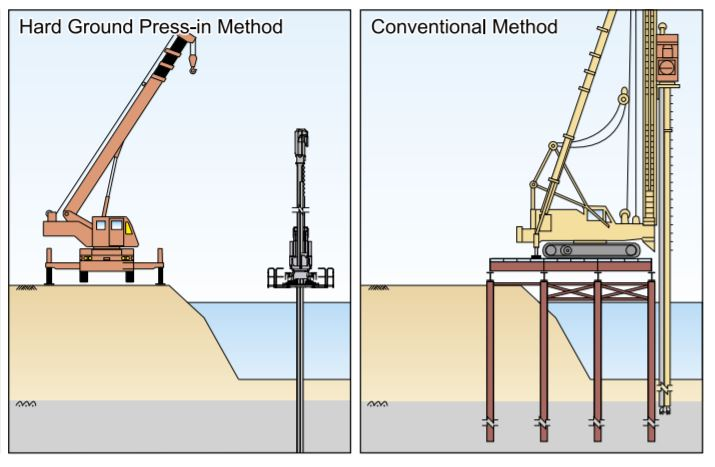
\includegraphics[height=.18\textheight]{pressin}
  	\captionsetup{justification=centering}
  	\caption{}
  	
	\label{magSim1}
	\end{center}
  \end{subfigure}
  \begin{subfigure}[h]{.5\textwidth}
  \begin{center}
  	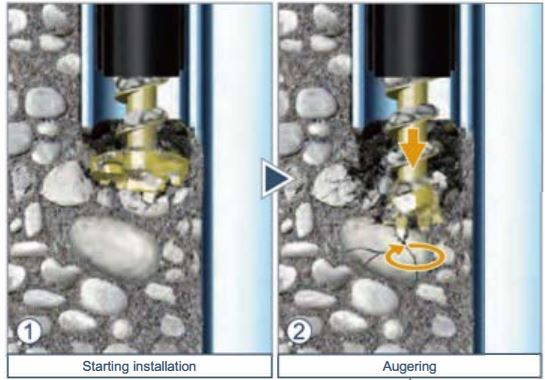
\includegraphics[height=.18\textheight]{supercrush}
  	\captionsetup{justification=centering}

\caption{}
  	\label{magSim2}
  \end{center}
  \end{subfigure}
  \caption{Diagram showing ability of Ivor King to pile from the land without additional foundations (a) and showing concept behind the Super Crush mechanism (b). \cite{l}  }
	\label{drills}
\end{figure}


Figure \ref{noise} shows a graph that displays the reduction in noise level with increasing distance from the source. It is stated that the pressing rigs produce 60-75 dB of noise on average \cite{m}, however due to the combined auguring, I have assumed that this rig will produce around 90dB. Some simple calculations shown below show that the noise level of this machinery will not exceed that of a residential area (35dB) \cite{m}, bearing in mind the closest residential area is about 470m from the site.
\end{justify}
\begin{figure}[H]
\centering
  	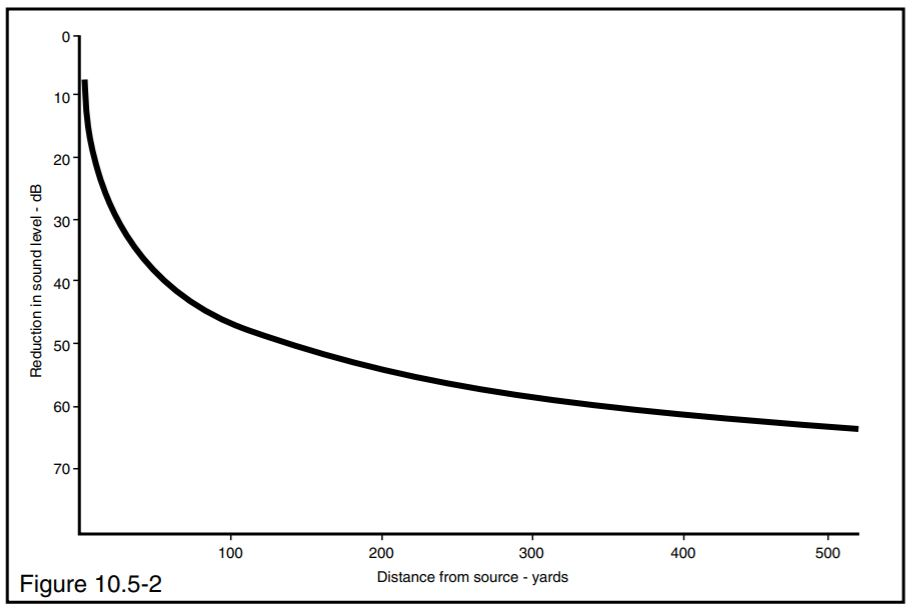
\includegraphics[width=0.5\textheight]{noise}
   	\caption{Graph to show how noise reduction varies with distance from the source.\cite{m}}
	\label{noise}
\end{figure}
\begin{equation}
    \text{400 yards}\implies \text{60\% reduction} 
\end{equation}
\begin{equation}
    0.40\times90dB=36dB\approx35dB
\end{equation}
\begin{justify}
Once all machinery is in place, the first task is to construct a template, to ensure that the wall is inserted perpendicular to the water. Figure \ref{temp} shows an example of how a template can be formed when piling on water. The chosen piling method is `Panel Driving', with Figure \ref{paneldriving} showing this process. The alternative is `pitch and drive', which although is a quicker process, is much less accurate in ensuring the piles are driven straight. The panel driving method is slower, but more accurate. Due to the lack of time pressure for this project, a slower method is acceptable. However, to speed up this process the piles can be pre-ordered in crimped pairs. This also makes the toe of the piles more durable and reduces the chance of the toe deforming when in contact with the sandstone. From Figure \ref{drive}, it can be seen that for hard driving conditions such as this site, and for piles of 10m, it is recommended that panel driving in pair is used, and that a section AZ18-800 is required. Although the design in this report is using AZ18-700 and is of 9m, this is very similar to the requirements just mentioned and thus it has been decided that this is the piling method to use. 
\end{justify}
\begin{justify}
The first pile is partially driven downwards. The remaining piles are pitched into place, within the template, and the last pair is also partially driven down. The remaining piles of the first panel are then driven down, working backwards from the last pair. Once the first panel is complete, the next panel is pitched, and the last pair of the first panel becomes the first pair of the second panel. The first panel is then driven down to the final depth in stages. Once this is complete, the second panel is partially driven using the same process as before, and this continues for the entire length of wall.
\end{justify}
\begin{justify}
From the drawings it is seen that the front wall is embedded to a depth of 3m, and the anchor wall to a depth of 1.5m. These are larger than the calculated depths, which are detailed earlier in this report. This is due to the auguring of rock reducing the strength, and thus the piles are taken to a depth slightly larger than the calculated depth to account for this. The extended depth also ensures that tolerances for the machinery are accounted for, as the piling machinery is unable to pile exactly to the nearest mm. 
\end{justify}

\begin{justify}
A sealant is not required for this project, as the active side is retaining soil, not water, and any water leakage will be minor. Any holes needed to slot the tie rods through will be pre-burned off site. Further to this, drainage holes are also pre-burned. These holes will ensure no excessive water buildup occurs behind the wall in times of peak rainfall. Burning the holes off-site is a health and safety consideration, to ensure that someone does not have to be in a precarious position with a dangerous piece of equipment on site. 
\end{justify}
\begin{figure}[H]
\centering
  	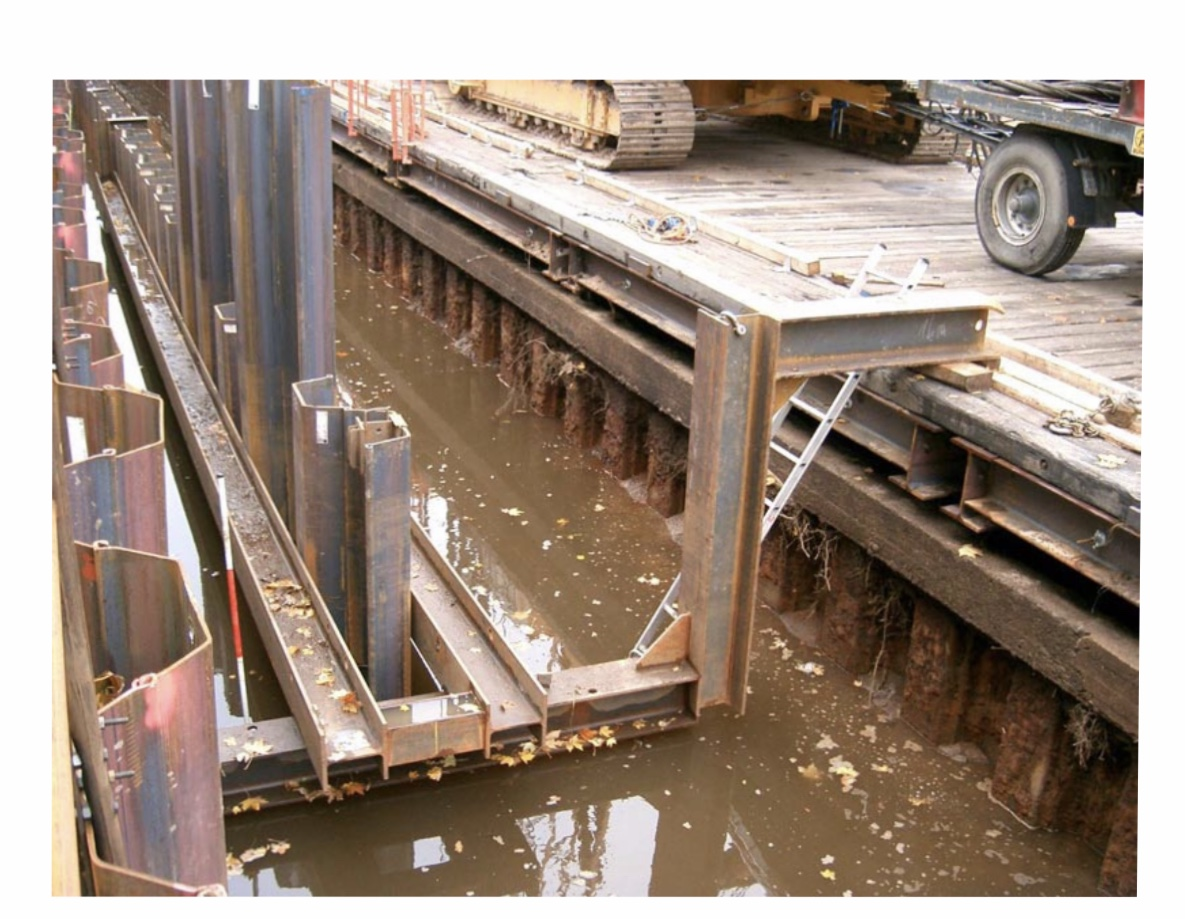
\includegraphics[width=0.5\textheight]{temp}
   	\caption{Example of water based template for sheet piles. \cite{m}}
	\label{temp}
\end{figure}  
\begin{figure}[H]
\centering
  	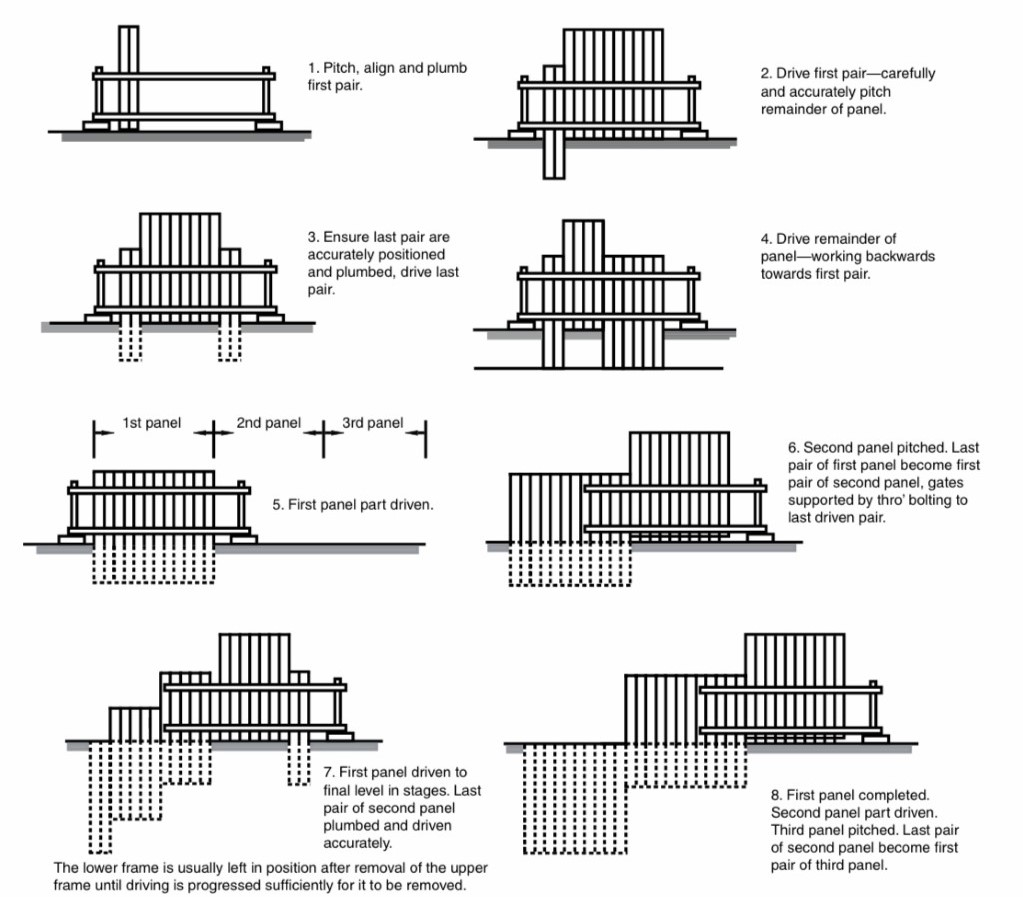
\includegraphics[width=0.4\textheight]{paneldriving}
   	\caption{Panel Driving process. \cite{m}}
	\label{paneldriving}
\end{figure}     
 \begin{figure}[H]
\centering
  	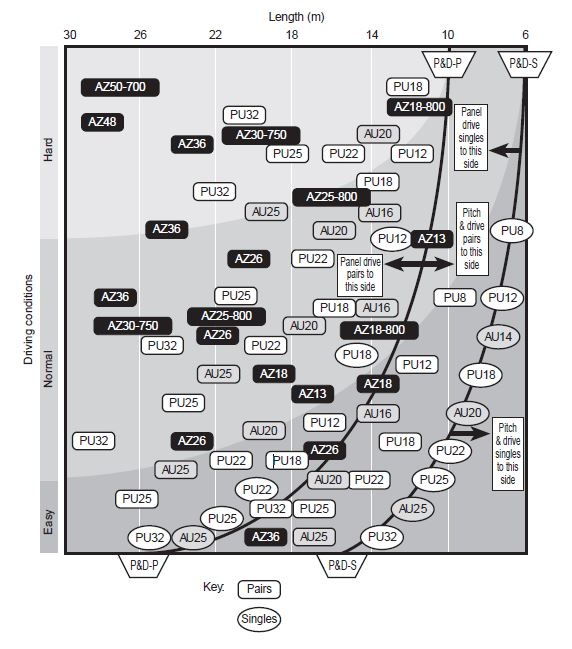
\includegraphics[width=0.4\textheight]{drive}
   	\caption{Graph to show the drivability of different sheet pile sections using different methods. \cite{d}}
	\label{drive}
\end{figure}     
                               
\begin{justify}
 Once the front wall has been fully embedded to the required depth, the next task is to remove the original buttresses and deck, which lie just behind the new wall. Following this the back filling of the wall will take place, to a level 0.5m below the level of the tie rods. This fill is to be compacted to minimise the chance of the concrete deck subsiding and cracking.  
\end{justify}
\subsection{Tie Rods and Bolts}
The next task is to cut slots down into the old concrete wall, to allow for the tie rods to pass through. This localised cutting allows for the existing wall to remain in place, not only saving time with removal, but also reducing the chance of wall failure by not applying the full load of the ground before the anchor is in place. A diamond chainsaw is ideal for cutting long slots into the concrete. 
\begin{justify}
Having done this, the next task is to dig a trench 2.0m down, from the existing wall to the start of the bank. This allows for the rock tie to be attached later on. Once the trench is dug, the anchor wall is to be inserted, as down previously with the main wall. Once this is inserted, the tie rods can be lined up between the main wall and anchor wall. The rods are bolted on to the front and back waling wall. The rods are then tightened at the turnbuckle, until taught.
\end{justify}
\subsection{Capping Beam}
\begin{justify}
At this point, both walls are embedded, and the tie rods are in place. The capping beam now needs to be formed. A wooden box template is constructed around the top of the sheet pile, allowing a portion of sheet pile to be embedded within the beam. Once the reinforcement cage has been tied together, it can be lifted into the wooden template. Concrete is then poured into the box, covering the rebars. The concrete is then given time to set. The original road is relaid with tarmac, ensuring that drainage is added, which carries any rain water inland, to ensure that there are no contaminants being flushed into the river.
\end{justify}
\begin{justify}
The final task is to cover up the tie rods with fill, and bring the ground surface back to its original level. A concrete deck is then laid on the compacted fill, between the road and the main wall. The final finishes are added, including a permanent safety rail to the deck, and drainage along the deck which will funnel any runoff inland.
\end{justify}
\subsection{Estimated time of construction}
\begin{justify}
The total length of wall to be constructed is 76m, which leads to 109 individual piles needed for the main wall and the anchor wall. A total of 31 tie rods are required. The below calculations break down the required time for embedding the piles and attaching the tie rods.
\end{justify}
\begin{equation}
    \text{Total length of embedment for front wall}=9\times109=981m
\end{equation}
\begin{equation}
    \text{Total length of embedment for anchor wall}=4\times109=436m
\end{equation}
\begin{equation}
    \text{Total length of sheet piles}=981+436=1417m
\end{equation}
\begin{align*}
    \text{Piling Rate per machine}=100\hspace*{0.1cm}\text{m/day}
\end{align*}
\begin{equation}
    \text{Number of days for piling}=\frac{1417}{100}=14.2 \hspace*{0.1cm} \text{days}
\end{equation}
\begin{align*}
    \text{Rate of tie rod installation}=2\hspace*{0.1cm}\text{rods/day}
\end{align*}
\begin{equation}
    \text{Number of days for tie rod installation}=\frac{31}{2}=15.5\hspace*{0.1cm}\text{days}
\end{equation}
\begin{table}[H]
    \centering
    \begin{tabular}{|c|c|c|}
    \hline
      &\textbf{Construction Activity}&\textbf{Time Taken} \\ \hline
     1. &Site Preparation&7\\ \hline
      2.&Piling&14.2 \\ \hline
      3.&Removal of Original Buttress and Deck&2\\ \hline
       4.&Waling Beam&5\\ \hline
      5.&Cutting Original Wall &2 \\ \hline
      
      6.&Tie Rods&15.5 \\ \hline
      7.&Capping Beam &14 \\ \hline
     & TOTAL&59.7\\ \hline
     &TOTAL with 10\% downtime for machines&66 \\ \hline
    \end{tabular}
    \caption{Estimated Time of Construction}
    \label{time}
\end{table}
\begin{justify}
From Table \ref{time} it can be seen that the project is expected to taken 66 days to complete from start to finish. The capping beam estimate is taking into account curing time as well as the time to build the reinforcement cage. 
\end{justify}
\section{Project Costing}
\begin{justify}
The estimated cost for the main components of the design are displayed in Table \ref{cost} below. Preliminary costs account for things such as setting up the plant, equipment, supplies and services. This is taken to be higher than the average small scale project due to the fact that specialist piling machinery is required. 
\end{justify}
\begin{table}[H]
    \centering
    \begin{tabular}{|c|c|c|c|}
    \hline
      \textbf{Component}&\textbf{Quantity}&\textbf{Rate}&\textbf{Cost (£)} \\ \hline
      Concrete&22.8 m$^3$&150\hspace*{0.1cm}£/m$^3$&3420 \\ \hline
      Waling Beam&7.3 tonnes&500\hspace*{0.1cm}£/ton&3635 \\ \hline
      Piles&108.4 tonnes&500\hspace*{0.1cm}£/ton&54,200 \\ \hline
      Tie Rods&6.2 tonnes&1500\hspace*{0.1cm}£/ton&9240 \\ \hline
      Fill&3928 tonnes&15\hspace*{0.1cm}£/ton&58,920 \\ \hline
      Rebars&2.9 tonnes&500\hspace*{0.1cm}£/ton&1446 \\ \hline
      & & TOTAL:&130,861\\ \hline
    \end{tabular}
    \caption{Estimated Cost of Materials}
    \label{cost}
\end{table}
\begin{align*}
\hspace*{1.7cm}
   \text{Preliminary Cost}=\text{£50,000}
\end{align*}
\begin{align*}
    \text{Ongoing plant and labour costs}=\text{£10,000 /week}
\end{align*}
\hrule
\begin{align*}
\hspace*{3.2cm}
    \text{Subtotal}=\text{£312,861}
\end{align*}
\hrule
\begin{align*}
\hspace*{0.6cm}
    \text{Contractors Profit (10\%)}=\text{£35,786}
\end{align*}
\begin{align*}
\hspace*{1.8cm}
    \text{Minor Items (5\%)}=\text{£15,643}
\end{align*}
\begin{align*}
\hspace*{1.6cm}
    \text{Contingency(10\%)}=\text{£35,786}
\end{align*}
\hrule
\begin{align*}
\hspace*{2.6cm}
    \text{TOTAL COST}=\text{£391,076}
\end{align*}
\section{Sustainability}
\subsection{Environmental}
\begin{justify}
One of the significant impacts to the environment is the carbon footprint associated with the manufacture and delivery of the materials. One solution to reduce this is to source all building supplies from local companies, to minimise the distance that materials have to travel. One advantage of the sheet piles over other concrete solutions is the ability to reuse the sheet piles. This means that although the carbon footprint per sheet pile is relatively high, in the long term the impact is less than the concrete alternatives due to the ability to reuse. ArcelorMittal, the supplier of the sheet piles, claim that piles can be reused between 3-10 times without losing their properties. Steel production produces 1770kg of CO$_2$/ tonne of steel produced \cite{n}, and concrete produces 180kg of CO$_2$/tonne of steel produced \cite{o}. However if the steel produced can be reused 10 times, then the argument for steel becomes a lot more attractive, with CO$_2$ production falling to 177kg/tonne of steel. It has therefore been important to use standard details in the design, to increase the chances that the sheet piles can be reused in future. If reusing is not an option, the piles can easily be melted down in electric arc furnaces for the steel to be used elsewhere. The Super Crush piling machine to be used has a new engine that `conforms the emission level to the Off Road Act \cite{l}'. The use of an electronically controlled fuel injection system reduces the amount of white and dark smoke produced from the engine during piling, all of which reduces the emissions from this project.
\end{justify}
\begin{justify}
A second environmental impact with this project is the potential threat to marine wildlife. It has been found that noise and vibrations (such as those from the Vibro Displacement piling machinery) can be incredibly harmful to fish, where organs can be damaged and haemorrhages can occur, killing large numbers very quickly. The fact that this project used press in piling techniques removes this threat. The Giken Super Crush piling machine to be used runs off a special biodegradable oil unique to Giken. The biodegradable nature means that if any is to spill onto the surrounding land, it will naturally decompose and thus cause no further issues for the local ecosystems. This oil has also passed the Fish Toxicity Text- 100\% of fish survived after 4 days in water which was containing the oil \cite{l}.
\end{justify}
\subsection{Social}
The local residents to this site have been considered throughout the design process, not only trying to minimise disturbance, but also trying to maximise their enjoyment of the final build. As discussed, noise levels have been considered, and it has been concluded that there will be no concern with the noise due to the use of silent press in technology. The delivery of machinery and materials is to be done at off peak times to minimise the impact to the local traffic. The focus with this project has been to provide a safe area which people can come to enjoy the waterfront, whether that is fishing from the deck, or dog walking. Safety rails have been implemented to uphold safety and benches have been added to maximise the enjoyment of visitors. 
\subsection{Economic}
\begin{justify}
The main economic benefit from this project is that local construction businesses will gain some work. This is excellent for the local economy, and could provide further projects for the contractors involved if a good job is done.
\end{justify}
\section{Final Design Conclusions}
\begin{justify}
A complete and justified design has been laid out in this report, with the full design seen in the drawings attached to this report. The main concern with this site was the contamination from past industry. As a result, the retaining wall design had to minimise excavation near the river, and as such sheet piles were chosen. The geology of this site posed an issue to the embedment process, with a dominant layer of hard sandstone beneath the ground with which the piles are to be driven into. This was solved by finding specialist equipment called the Giken Super Crush Piler, which not only deals with the issue of the rock, but also carries out the piling with minimal noise. 
\end{justify}
\begin{justify}
The construction sequence has been considered, arriving at an estimated project time of 66 days. This time is the best case solution however, with obvious delays occurring if there is bad weather. An estimate of the project cost came to £391,076. This is clearly a considerable cost, however it is a required cost to ensure that no one is harmed by the currently dangerous site.
\end{justify}

\begin{thebibliography}{}
\bibitem{a}Butcher, L. (2009). Lorry sizes and weights. [ebook] House of Commons Library. Available at: https://researchbriefings.files.parliament.uk/documents/SN00654/SN00654.pdf [Accessed 29 Jan. 2020].
\bibitem{b}Maloney's Quay Wall Project Specification. (2019). Durham University Engineering Department.
\bibitem{c}Union of Concerned Scientists. (2017). Coal and Water Pollution. [online] Available at: https://www.ucsusa.org/resources/coal-and-water-pollution [Accessed 3 Feb. 2020].
\bibitem{d}Piling Handbook. (2016). 9th ed. Luxembourg: Imprimerie Centrale.
\bibitem{e}Knappett, J., \& Craig, R. F. (2012). Craig's soil mechanics. Retrieved from https://ebookcentral.proquest.com
\bibitem{f}Sections-Parallel Flange Channels (PFC). (n.d.). [ebook] Available at: https://britishsteel.co.uk/media/40513/british-steel-universal-beams-pfc-datasheet.pdf [Accessed 5 Mar. 2020].
\bibitem{g}ASDO. (n.d.). M12 – M160 ARCHITECTURAL STRUCTURAL TIE BARS in accordance with EN1993-1. [online] Available at: http://pretec.no/wp-content/uploads/2016/05/ASDO-brochure-englisch$$_$$5MB.pdf [Accessed 5 Mar. 2020].
\bibitem{h}BSI British Standards-UK National Annex to Eurocode 3: Design of steel structures – Part 5: Piling. (2009). 
\bibitem{i}Wells, J. (2009). Design Of Capping Beams. The Structural Engineer 87.
\bibitem{j}Draycott, T. (2009). Structural elements design manual. 2nd ed. Oxford: Elsevier, pp.Table 3.15.
\bibitem{k}Managing health and safety in construction Construction (Design and Management) Regulations 2015. (2015). [ebook] Available at: https://www.hse.gov.uk/pubns/priced/l153.pdf [Accessed 6 Mar. 2020].
\bibitem{l}Ivor King(2010). Hard ground press in method- The silent piler for hard ground-Technical Brochure. 
\bibitem{m}NASSPA Best Practices Sheet Piling Installation Guide. (2005). North American Steel Sheet Piling Association.
\bibitem{n}greenspec. 2020. Steel Production & Environmental Impact. [online] Available at: <http://www.greenspec.co.uk/building-design/steel-products-and-environmental-impact/> [Accessed 11 March 2020].
\bibitem{o}A. Samarin (7 September 1999), "Wastes in Concrete :Converting Liabilities into Assets", in Ravindra K. Dhir; Trevor G. Jappy (eds.), Exploiting wastes in concrete: proceedings of the international seminar held at the University of Dundee, Scotland, UK, Thomas Telford, p. 8, ISBN 9780727728210.




\end{thebibliography}
\appendix
\begin{appendices}
\section{Ground profile along length of wall}
\begin{figure}[H]
  \centering
  	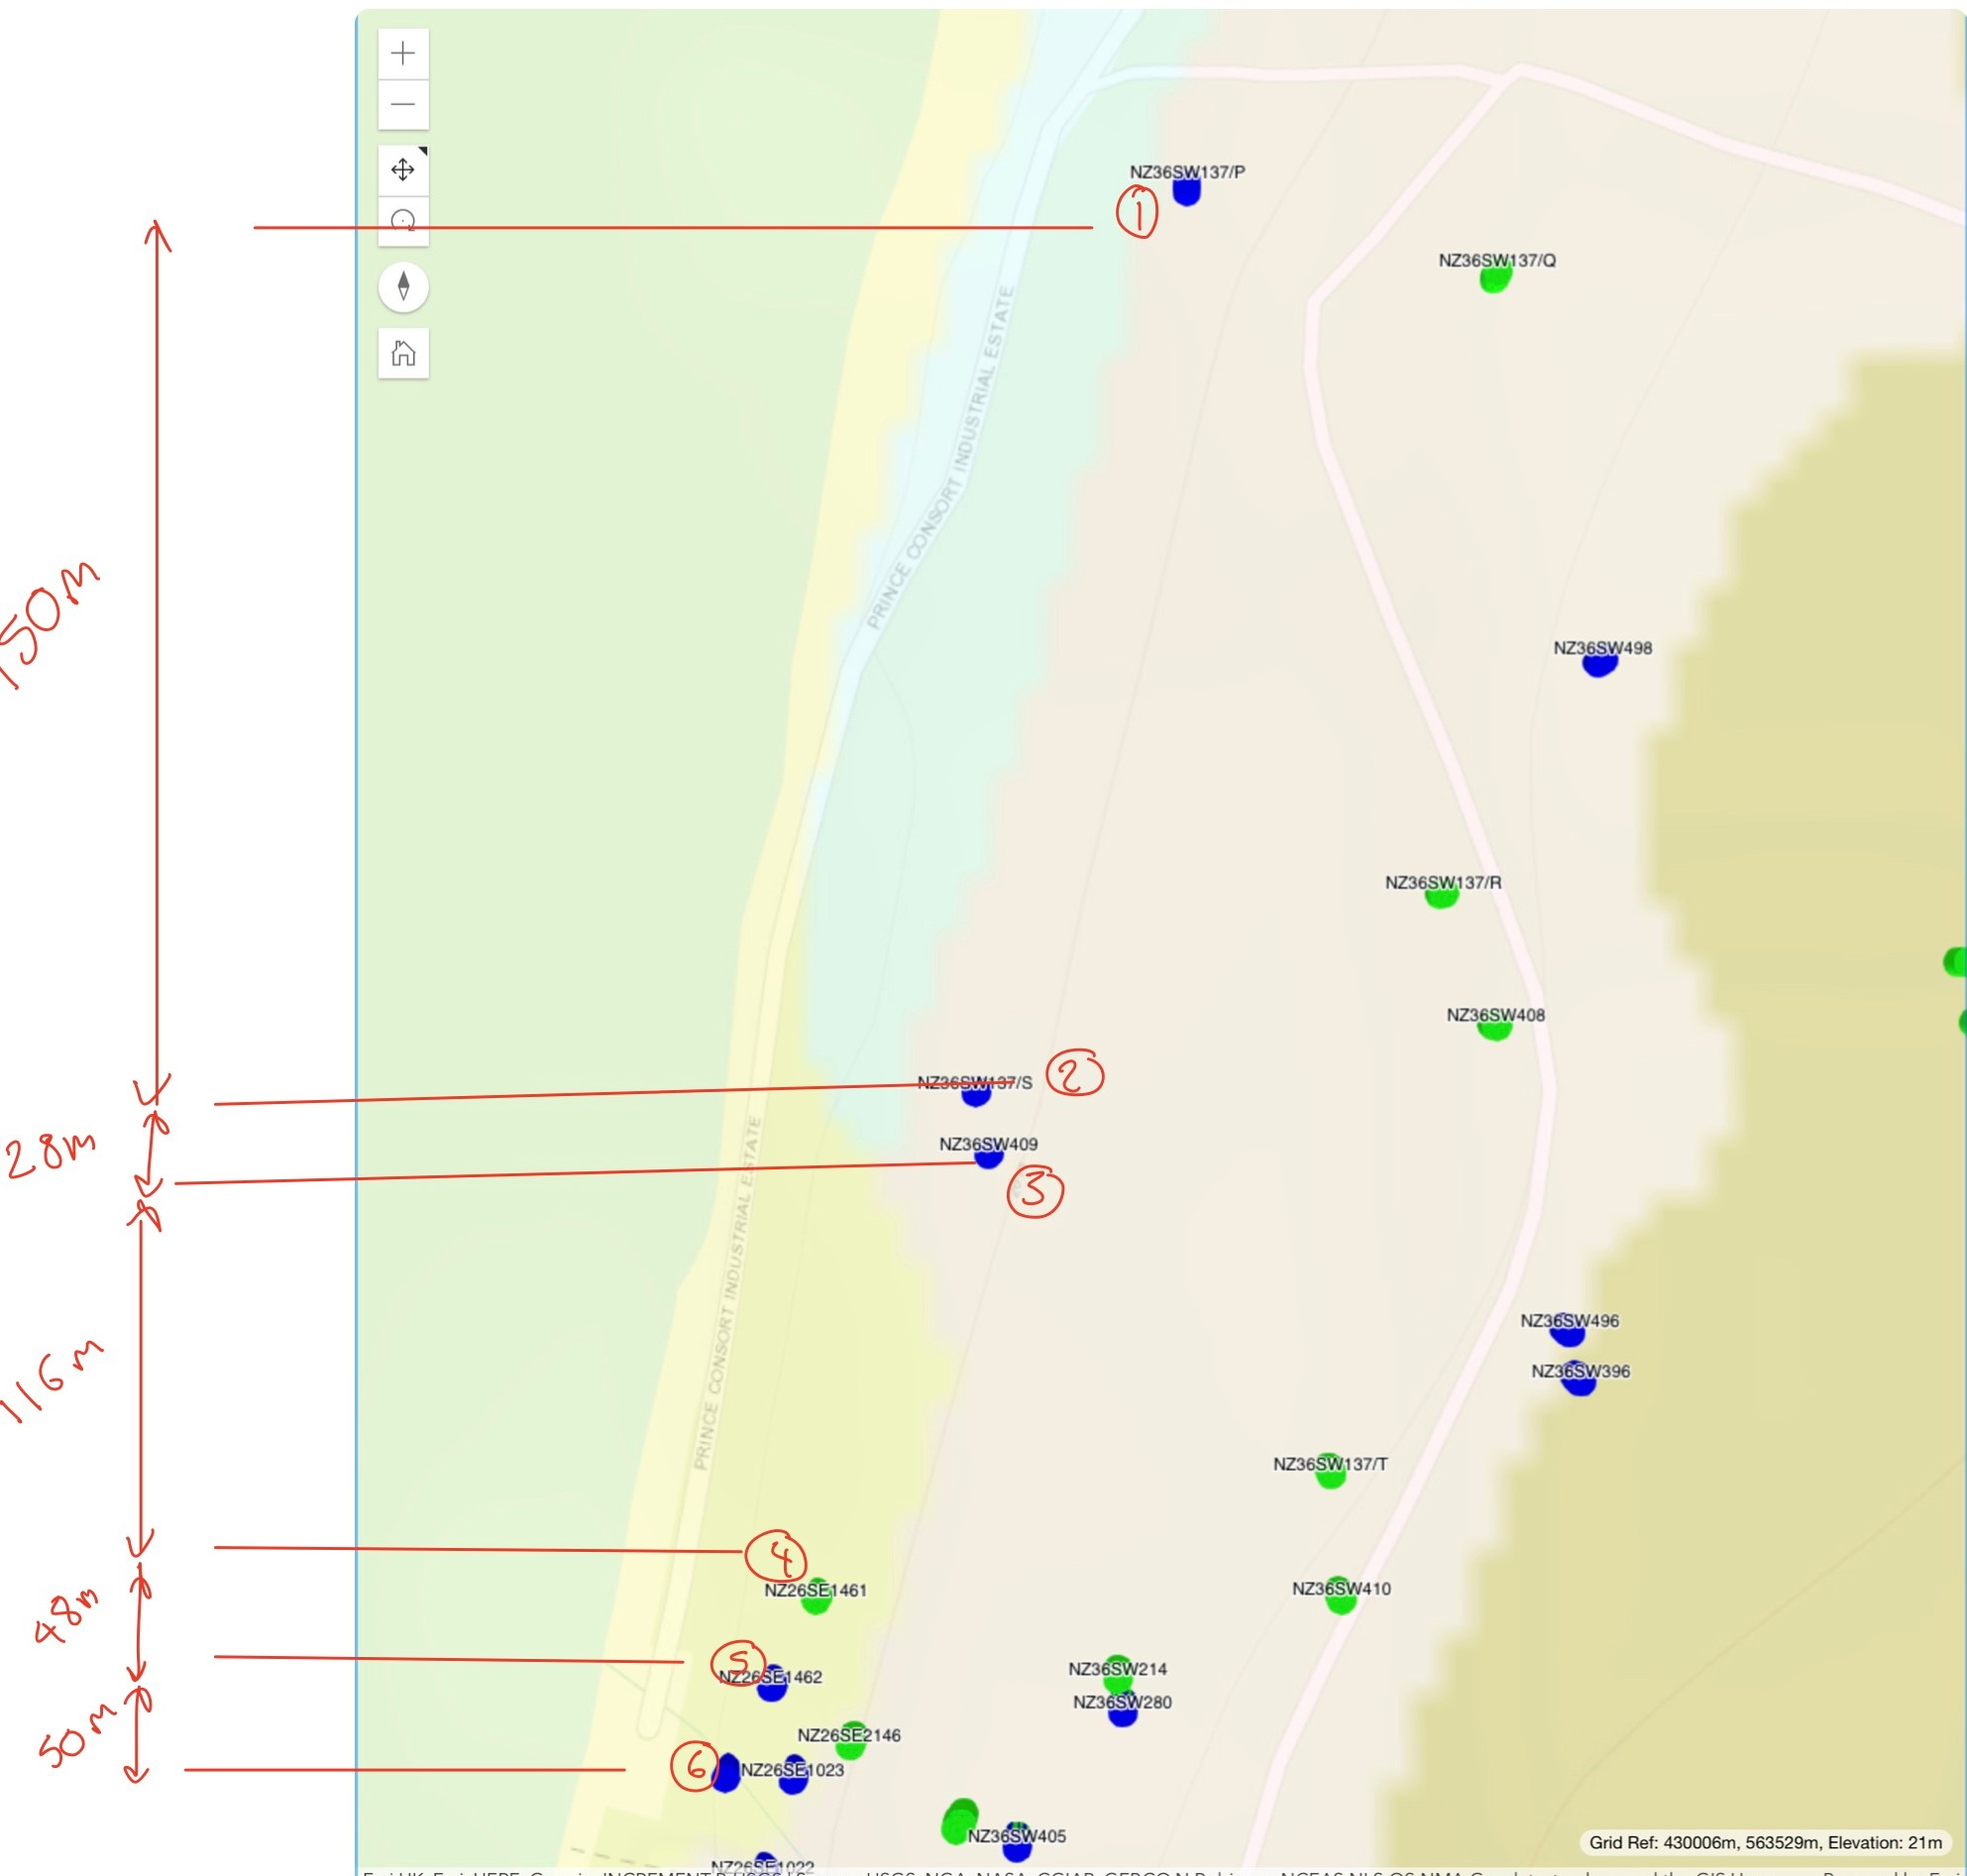
\includegraphics[width=0.5\textheight]{key}
   	\caption{}
	\label{length}
\end{figure}

\begin{figure}[H]
  \hspace*{-1.65cm}
  	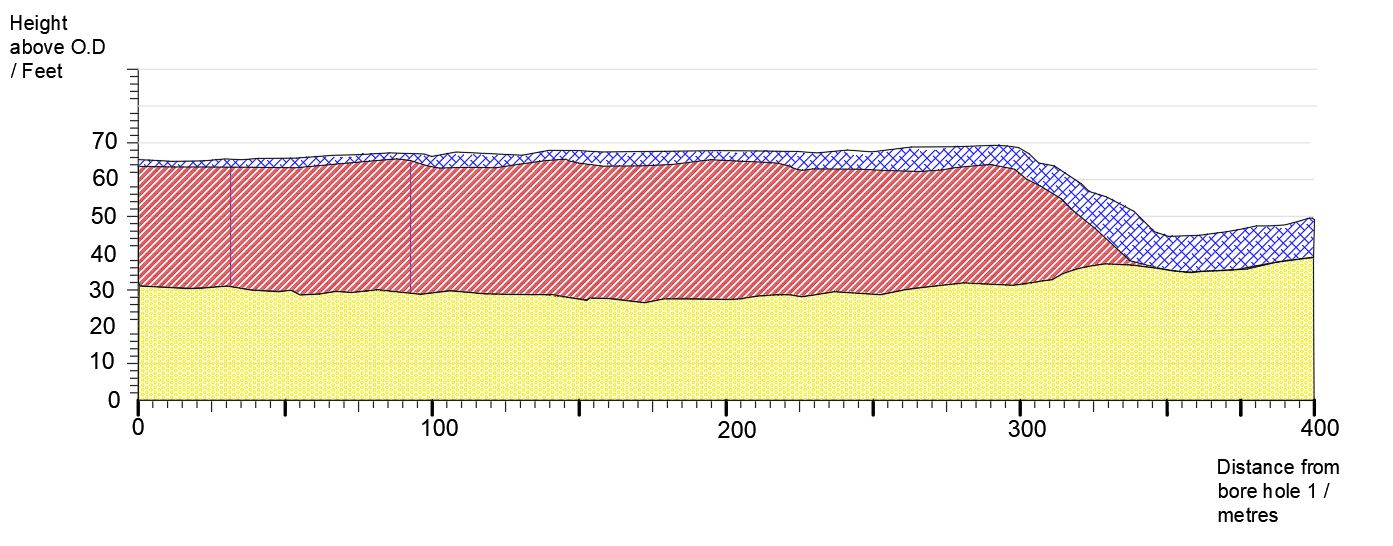
\includegraphics[width=0.8\textheight]{groundprof}
   	\caption{}
	\label{length}
\end{figure}

\section{Design Matrix}
\begin{figure}[H]
  \centering
  	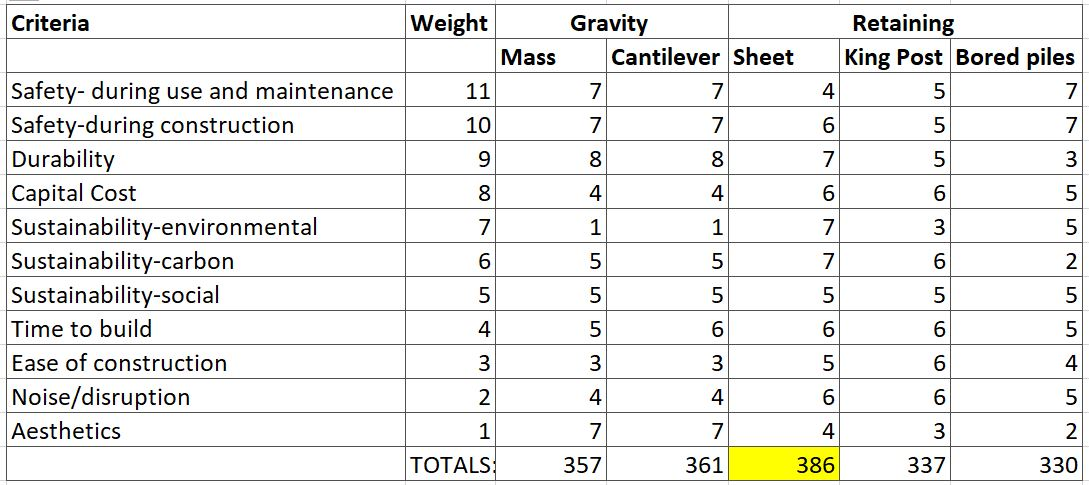
\includegraphics[width=0.5\textheight]{designmatrix}
   	\caption{}
	\label{length}
\end{figure}
\section{Details of Initial Active and Passive earth pressure, without rock tie}

\begin{figure}[H]
\hspace*{-1cm}
  \centering
  	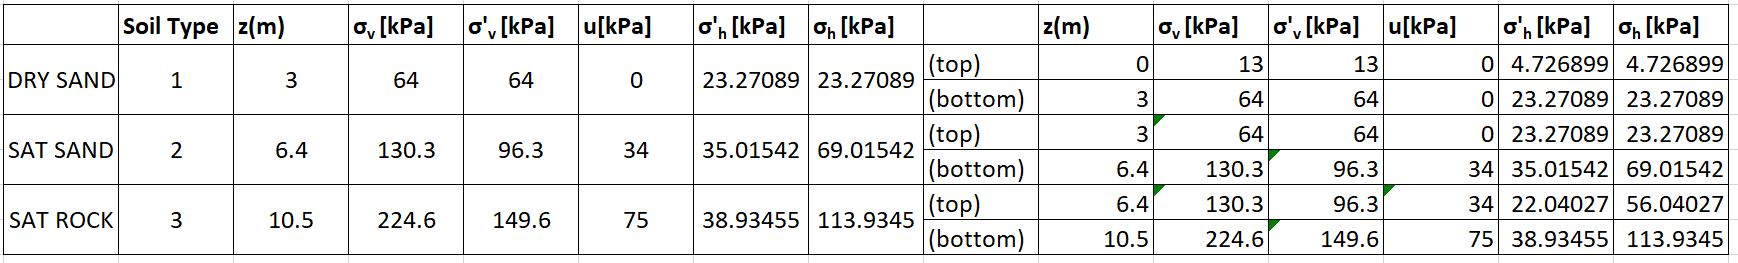
\includegraphics[width=0.75\textheight]{initialhorizstress}
   	\caption{Active Soil Pressure Calculations}
	\label{actinit}
\end{figure}

\begin{figure}[H]
\hspace*{-1cm}
  \centering
  	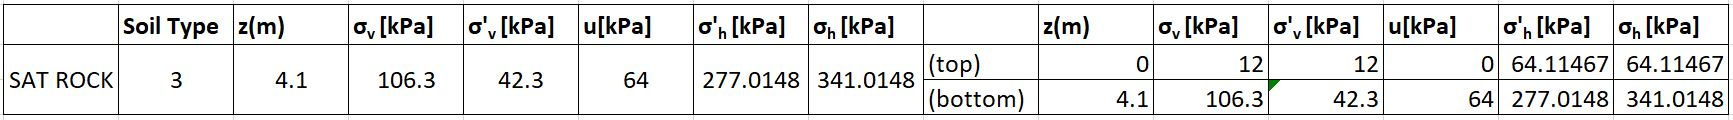
\includegraphics[width=0.75\textheight]{initialhorizstressPass}
   	\caption{Passive Soil Pressure Calculations}
	\label{passinit}
\end{figure}

\section{Details of the values used in moment calculations}
\begin{figure}[H]
\hspace*{-1cm}
  \centering
  	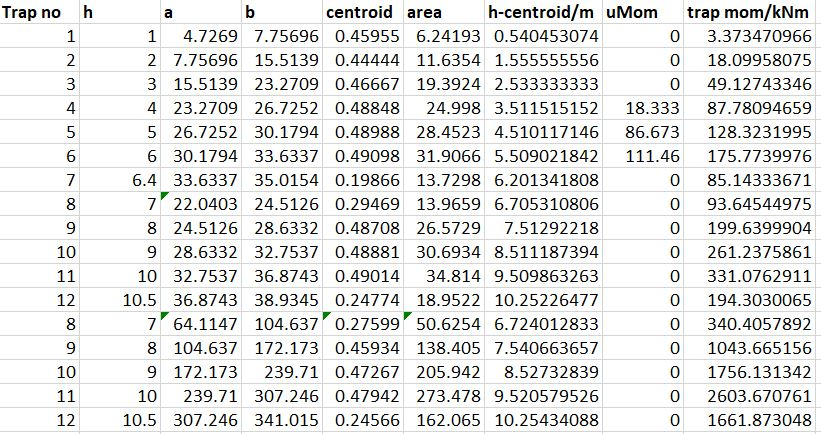
\includegraphics[width=0.75\textheight]{bendingmomentscalcstable}
   	\caption{Values used with no anchor}
	\label{bendmomtab}
\end{figure}
\begin{figure}[H]
\hspace*{-1cm}
  \centering
  	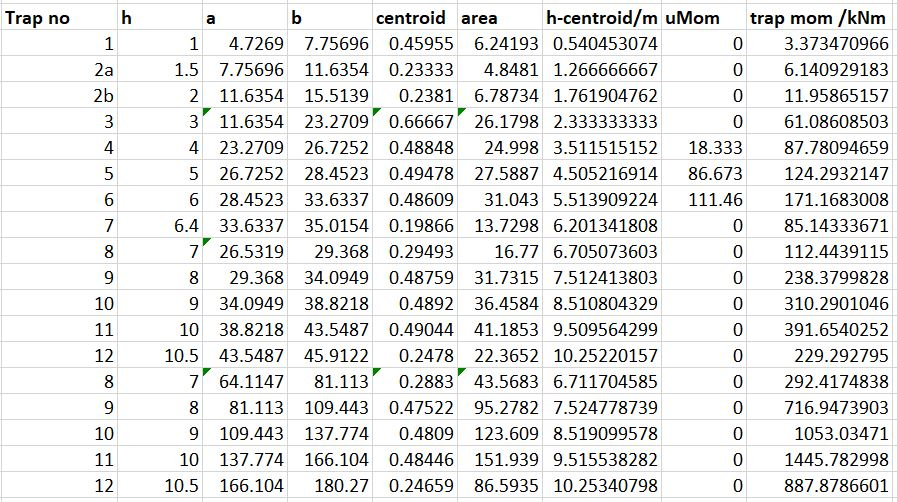
\includegraphics[width=0.75\textheight]{anchorbmcalcs}
   	\caption{Values used with anchor}
	\label{bendmomtab}
\end{figure}

\section{Tables used in determining the size of the Anchor Wall}

\begin{figure}[H]
  \centering
  	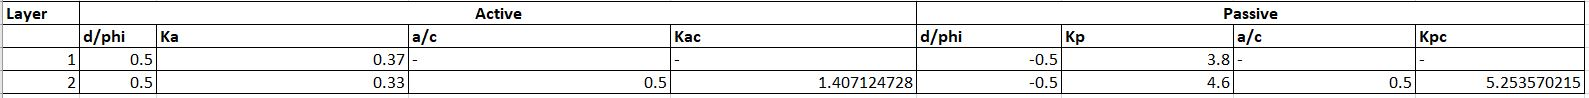
\includegraphics[width=0.7\textheight]{anchorwall1}
   	\caption{Soil Properties for Active and Passive sides of the anchor wall. NB d=$\delta$}
	\label{anchor1}
\end{figure}


\begin{figure}[H]
  \centering
  	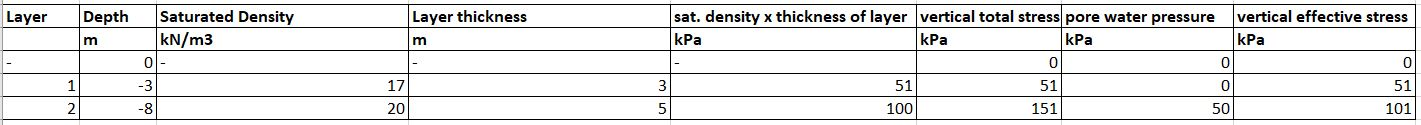
\includegraphics[width=0.7\textheight]{anchorwall2}
   	\caption{Vertical effective stress calculations, assuming anchor wall no deeper than 8m.}
	\label{anchor2}
\end{figure}



\begin{figure}[H]
  \centering
  	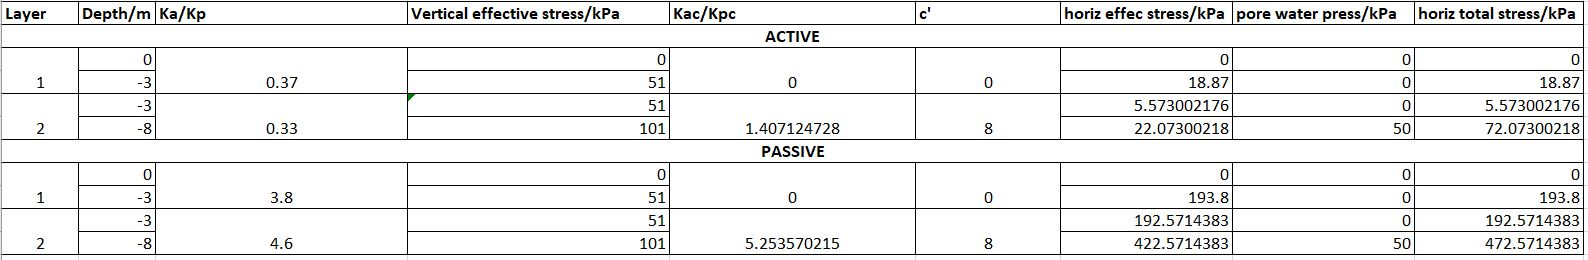
\includegraphics[width=0.7\textheight]{anchorwall3}
   	\caption{Horizontal total stress for both active and passive sides.}
	\label{anchor3}
\end{figure}




\begin{figure}[H]
  \centering
  	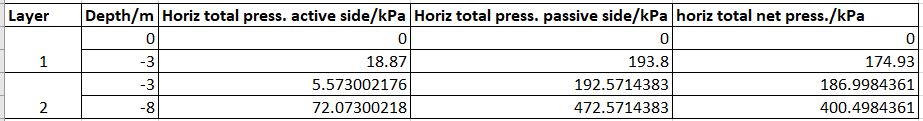
\includegraphics[width=0.7\textheight]{anchorwall4}
   	\caption{Net total horizontal stress on anchor wall.}
	\label{anchor4}
\end{figure}





\begin{figure}[H]
  \centering
  	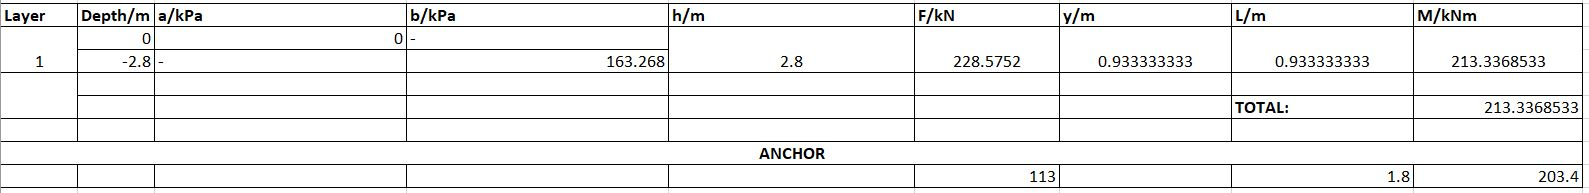
\includegraphics[width=0.7\textheight]{anchorwall5}
   	\caption{Moments taken about toe of anchor wall (assumed depth).}
	\label{anchor5}
\end{figure}

\begin{figure}[H]
  \centering
  	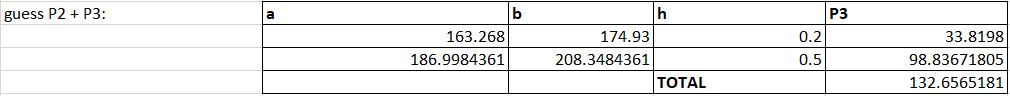
\includegraphics[width=0.7\textheight]{anchorwall6}
   	\caption{Values used to calculate the value of P2+P3 to find final anchor wall height.}
	\label{anchor6}
\end{figure}


\end{appendices}



\end{document}

